% Original template author: Joseph Rowell
% Version: 3.0
% This work is licensed under a Creative Commons Attribution 4.0 International License.
\documentclass[12pt, a4paper]{report}
\usepackage[a4paper, total={6.25in, 8.25in}]{geometry} %%%%%% CHECK MARGIN REQ. 8.25 in?
\input{Packages.tex}
\usepackage{multicol}
\hypersetup{pdftitle = {Beyond Persona Prompting: A Cognitive-Process-Based Framework for ADHD Student Simulation with Large Language Models}, pdfauthor = {Qingqing Liu}, pdfstartview=FitH, pdfkeywords = {large language models, simulated students, ADHD, learner modelling, working memory}, pdfpagemode = FullScreen, colorlinks, anchorcolor = black, citecolor = blue, urlcolor = blue, filecolor = green, linkcolor = blue, plainpages = false}
%%%%%%%%%%%%%%%%%%%%%%%%%%%%%%%%%%%%%%%%%%%%%%%%%%%%%%%%%%%%%%%%%%%%%%%
\pagestyle{fancy}
\rhead{}
\chead{}
\lhead{University College London}
\lfoot{\date{}}
\cfoot{}
\rfoot{\thepage}
% Top and Bottom Line Rules

\renewcommand{\headrulewidth}{0.4pt} %0.4pt
\renewcommand{\footrulewidth}{0.4pt}
\fancyheadoffset{8pt}
\fancyfootoffset{8pt}
% Line spacing
\renewcommand{\baselinestretch}{1.5} %1.5

\date{September 1, 2026}

\title{Beyond Persona Prompting: \\ A Cognitive-Process-Based Framework for ADHD Student Simulation with Large Language Models}
\author{\\ \Large{Qingqing Liu}
\\ Student Number: 25098690
\\ Supervisor: Dr Sahan Bulathwela
\\ Faculty of Engineering
\\ Department of Computer Science
\\ 
\\
\\ University College London
\\
A Project Report Presented in Partial Fulfilment of the Degree \\ \textit{MSc Artificial Intelligence for Sustainable Development}
\\ \\
}
%%%%%%%%%%%%%%%%%%%%%%%%%%%%%%%%%%%%%%%%%%%%%%%%%%%%%%%%%%%%%%%%%%%%%%%
\begin{document}
%Adjust logo positions here
% \AddToShipoutPicture*{\parbox[t][\paperheight][t]{\paperwidth}{%
%           \includegraphics[width=\paperwidth]{\BackgroundPicturea{Logos/ucl_long%_logo.png}{3in}{3in}}
%           }}
% \AddToShipoutPicture*{\centering\BackgroundPictureb{Logos/Bentham2011_065_c623d.jpg}{3in}{3.7in}}
\AddToShipoutPictureBG*{%
  \AtPageUpperLeft{%
    \raisebox{-\height}{%
      
\includegraphics[width=\paperwidth]{Logos/UCL page header.png}%
    }}
}
\AddToShipoutPicture*{%
      \parbox[t][\paperheight][t]{\paperwidth}{%
          
\includegraphics[width=1.2\paperwidth]{Logos/UCL page footer.png}
      }}
      

\thispagestyle{headings}
\maketitle
\FloatBarrier
\pagenumbering{roman}

\thispagestyle{empty}
\begin{abstract}
Large Language Models (LLMs) enable flexible student simulation through natural-language persona prompting, but descriptive learner profiles do not necessarily reproduce the learning-process consequences implied by process-relevant characteristics. This thesis investigates whether selected ADHD-related learning characteristics can instead be represented through explicit cognitive-process constraints that shape learner state and downstream behaviour.

A Cognitive-Process-Based (CPB) framework was developed to operationalise susceptibility to controlled distraction and sensitivity to instructional processing demand through Attention- and Working-Memory-related constraints. CPB was compared with persona-prompted student simulation using shared instructional materials, assessment questions, and a source-grounded criterion-level evaluation framework.

Three studies evaluated the approach. Study 1 verified that CPB mechanisms executed as intended and produced traceable information-state changes. Study 2 found that CPB produced clearer graded learner-condition patterns and more theory-consistent sensitivity to controlled distraction and processing demand than persona prompting. Study 3 showed that additional response-stage Language Ability and Big-Five prompts changed assessment outcomes but did not eliminate CPB's previously established constraint-related aggregate patterns.

These findings support functional process-based representation as a promising approach for modelling selected ADHD-related learning characteristics, while not claiming a complete or clinically valid simulation of ADHD cognition.


\keywords{large language models - simulated students - ADHD - learner modelling - working memory}
% \vspace{-10mm} %To remove added white space after
\end{abstract}
\newpage
\thispagestyle{empty}
\vspace*{\fill}
\begin{center}
Copyright \copyright  \thinspace 2026 by Qingqing Liu \\ All Rights Reserved
\end{center}
\vspace*{\fill}
\newpage


\thispagestyle{empty}
\chapter*{Acknowledgements}


\thispagestyle{empty}
\chapter*{Declaration}
I, Qingqing Liu, declare that the thesis has been composed by myself and that the work has not been submitted for any other degree or professional qualification. I confirm that the work submitted is my own, except where work which has formed part of jointly-authored publications has been included and referenced. The report may be freely copied and distributed provided the source is explicitly acknowledged.\par
%Add signature png here.
% \begin{figure}[H]
% \includegraphics{Logos/signature.PNG}
% \end{figure}
\vspace{1.2cm}
\noindent\begin{tabular*}{\textwidth}
{@{}l@{\hspace{0.2cm}}p{0.38\textwidth}
@{\hspace{0.8cm}}
l@{\hspace{0.2cm}}p{0.38\textwidth}@{}}
\textit{Signature:} & \underline{\makebox[\linewidth]{}} &
\textit{Date:} & \underline{\makebox[\linewidth]{September 1, 2026}}
\end{tabular*}



\tableofcontents

\thispagestyle{plain}
\listoffigures
\listoftables
%\lstlistoflistings
\listofalgorithms


%\begin{singlespace}
\chapter*{List of Abbreviations}
\begin{sortedlist} %sort alphabetically
  \sortitem{ADHD:    Attention-Deficit/Hyperactivity Disorder}
  \sortitem{CPB:     Cognitive-Process-Based}
  \sortitem{LLM:     Large Language Model}
  \sortitem{LTM:     Long-Term Memory}
  \sortitem{NT:      Neurotypical}
  \sortitem{PDB:     Processing Demand Bits}
  \sortitem{RQ:      Research Question}
  \sortitem{WM:      Working Memory}
  \end{sortedlist}
% \end{singlespace}
%%%%%%%%%%%%%%%%%%%%%%%%%%%%%%%%%%%%%%%%%%%%%%%%%%%%%%%%%%%%%%%%%%%%%%%%%%%%%%%%
\pagenumbering{arabic}
\chapter{Introduction} \label{Chap1}

\section{Background and Motivation}

Simulated students have long been used in teacher training, intelligent tutoring-system development, and research on learning behaviour. The open-ended language generation, multi-turn interaction, and natural-language conditioning capabilities of large language models (LLMs) have further expanded the scope of student simulation, allowing simulated learners to participate in more flexible classroom dialogue, answer open-ended questions, and display different interactional characteristics according to predefined learner profiles \cite{markel-etal-2023-gpteach,liu-etal-2024-personality,chu-etal-2025-llm}. These developments make LLM-based student simulation increasingly relevant not only to teacher rehearsal, but also to tutoring-system testing and synthetic educational experimentation.

As simulated learners are increasingly used to compare teaching strategies, investigate learner differences, and analyse learning outcomes, however, generating natural or superficially plausible student responses is no longer sufficient to support stronger research claims. Recent studies show that LLM-simulated students can produce fluent dialogue while still deviating from the target learner in behavioural consistency, knowledge level, or cognitive fidelity \cite{martynova-etal-2025-can,scarlatos-etal-2026-simulated}. A more fundamental methodological question therefore arises: \textit{if simulated-learner behaviour is used to infer learning processes or compare learner conditions, the representation of learner characteristics directly determines how those behavioural differences can be interpreted}.

\section{The Representation Problem}

Persona prompting is one of the most direct and flexible approaches to learner representation in LLM-based student simulation. Characteristics such as academic ability, language ability, personality, motivation, and behavioural tendencies can be written into a prompt as natural-language profiles, after which the same foundation model adjusts its generated behaviour accordingly \cite{benedetto-etal-2024-using,liu-etal-2024-personality}. This approach requires no additional training and facilitates the rapid combination of multiple learner dimensions.

Learner characteristics do not necessarily operate at the same functional level, however. Some characteristics are expressed primarily through linguistic organisation, interactional tendencies, or response style. Others theoretically affect attention, information processing, or knowledge formation and therefore operate closer to the learning process itself. When these functionally heterogeneous characteristics are all represented through a single global persona prompt, the model can be told what the student is like or how the student should behave, but the way in which each represented characteristic enters the learning process and produces downstream behaviour remains implicit.

Persona prompting primarily constrains generated behaviour directly through descriptive learner profiles, whereas process-based representation allows selected learner characteristics first to act on the learning process, alter the learner state, and then influence downstream behaviour through the resulting state. The central distinction is therefore not whether behavioural variation is permitted, but whether behavioural differences are directly described or arise from preceding process constraints and the learner state that they form.

The central representation problem examined in this thesis is therefore whether descriptive persona conditioning is sufficient when learner characteristics are expected to affect knowledge acquisition and downstream task behaviour through the learning process, or whether those characteristics need to be represented at the processing level at which they are expected to operate.

\section{ADHD Student Simulation as the Research Case}

ADHD provides a useful case for examining this representation problem because many ADHD-related differences are expected to affect learning processes rather than only observable response style. At the same time, ADHD is highly heterogeneous: learners with the same diagnosis may differ substantially in cognitive profile and behavioural presentation \cite{willcutt-etal-2005-validity,luo-etal-2019-heterogeneity}. It would therefore be inappropriate to treat ``ADHD'' as a single fixed learner persona or to assume that one set of cognitive characteristics applies to all ADHD learners.

Rather than attempting to simulate ADHD as a whole, this thesis focuses on two bounded learning-related characteristics with established theoretical relevance. The first is \textit{susceptibility to controlled distraction}, reflecting the possibility that task-irrelevant events may disrupt the availability of task-relevant instructional information. The second is \textit{sensitivity to instructional processing demand}, reflecting the possibility that performance becomes more constrained as processing demands exceed available Working-Memory resources \cite{aboitiz2014irrelevant,martinussen2005meta,kofler2010adhd}. These characteristics are used as controlled functional targets rather than diagnostic markers or a complete cognitive model of ADHD.

Both characteristics are particularly suitable for the representation question examined here because their expected effects occur during learning: they concern what information remains available, how that information is processed, and what learner state is subsequently formed. They therefore provide a scoped test case for comparing a descriptive persona representation with a representation that places selected learner characteristics within the learning process itself.

To investigate this distinction, the thesis introduces a \textit{Cognitive-Process-Based} (CPB) learner representation. CPB represents the selected Attention- and Working-Memory-related characteristics as controlled processing constraints that shape the learner knowledge state, while persona prompting serves as the comparison representation. The subsequent studies examine whether these constraints operate as intended, whether they produce task behaviour consistent with the targeted processes, and whether the resulting constraint-related patterns remain observable when additional response-stage learner attributes are introduced.

\section{Research Aim, Research Questions and Objectives}

The aim of this thesis is to investigate whether selected ADHD-related learning characteristics can be represented as explicit and traceable processing constraints in LLM-based student simulation, and how this process-based representation differs from persona prompting in mechanistic validity, task-sensitive behavioural patterns, and multidimensional profile extension.

The study does not seek to establish that CPB is universally superior to persona prompting. Instead, it examines the forms of evidence that each representation can support under different functional claims: whether the CPB mechanisms affect the learner knowledge state according to their registered rules; whether the two representations produce different assessment-performance structures; and whether their behavioural patterns relate to controlled distraction and instructional processing demand in theoretically expected directions.

The following research questions address this aim.

\noindent\textbf{Main Research Question:} How can selected ADHD-related learning characteristics be represented in LLM-based student simulation, and to what extent does a cognitive-process-based representation produce more theory-consistent task behaviour than persona prompting while retaining its constraint-related patterns under additional response-stage learner attributes?

\noindent\textbf{RQ1---Mechanism:} Does the CPB processing pipeline execute its intended rules and produce traceable transitions from instructional information, through attention, working-memory processing and encoding, to Explicit LTM?

RQ1 first examines whether CPB itself operates as designed. Before final behaviour is compared, the study verifies whether the Attention and Working-Memory mechanisms execute correctly and whether the information-state changes caused by these mechanisms can be attributed and traced to the final Explicit LTM.

\noindent\textbf{RQ2---Representation:} Compared with persona prompting, does CPB produce learning behaviour that shows more theoretically consistent sensitivity to controlled distraction and instructional processing demand?

RQ2 then extends the analysis from the mechanism level to observable assessment behaviour. The study first compares learner-condition differentiation within each representation and then tests whether performance shows sensitivity to controlled distraction and source-round instructional processing demand in directions consistent with the targeted Attention- and Working-Memory-related hypotheses.

\noindent\textbf{RQ3---Constraint-Pattern Retention under Attribute Additions:} When Language Ability and Big-Five prompt dimensions are added at the response stage, how do assessment outcomes change, and do CPB's previously established constraint-related aggregate patterns remain observable?

RQ3 finally examines a more complex multidimensional learner representation. The addition of Language Ability and Big-Five prompt dimensions can reasonably change individual assessment responses, so the study does not require final outcomes to remain unchanged. The more important test is whether the graded performance structure and aggregate sensitivity to controlled distraction and instructional processing demand established for CPB remain observable after these response-stage attributes are introduced.

The three RQs therefore form a progressive sequence. RQ1 tests whether the process representation forms a traceable learner state through predefined mechanisms. RQ2 tests whether this representation subsequently produces theoretically relevant, task-sensitive behaviour. RQ3 then examines whether these constraint-related aggregate patterns remain observable after further learner-profile dimensions are added.

Four research objectives operationalise these questions:

\begin{enumerate}
    \item \textbf{Develop a process-based learner representation} that operationalises the selected ADHD-related Attention and Working-Memory characteristics as explicit processing constraints and represents the learner information formed after instructional experience in a separate knowledge state.
    \item \textbf{Validate the internal CPB processing pipeline} by testing whether the Attention and Working-Memory mechanisms execute according to their predefined rules and whether the corresponding information-state transitions are correct, attributable, and traceable to Explicit LTM.
    \item \textbf{Compare persona prompting and CPB at the behavioural level} by examining the within-representation performance structure of each approach and its sensitivity to controlled distraction and instructional processing demand.
    \item \textbf{Examine constraint-pattern retention under multidimensional profile additions} by analysing changes in assessment outcomes after Language Ability and Big-Five prompt dimensions are introduced and testing whether the established CPB constraint-related aggregate patterns remain observable.
\end{enumerate}

\section{Contributions}

This thesis makes three principal contributions across learner representation, validation methodology, and controlled empirical comparison.

\textbf{First, a functionally factorised learner-representation framework.} The thesis introduces CPB, which functionally distinguishes selected process-relevant learner characteristics from persona-style response attributes within the representation architecture. Rather than describing learner behaviour only through a natural-language persona, CPB allows some task behaviour to arise from controlled information-processing constraints and the learner knowledge state that they form. It thereby provides an alternative design for investigating how heterogeneous learner characteristics can be represented according to their functional roles.

\textbf{Second, a traceable and claim-matched validation framework.} The thesis separates learner-simulation validation into distinct evidential levels, including mechanism execution, information-state transition, learner-condition performance structure, process-sensitive behavioural response, and constraint-pattern retention. Through explicit intermediate states, source-grounded assessment criteria, and structured outcome evaluation, representation claims at different levels can be connected to observable and auditable evidence rather than relying on a single final realism or performance score.

\textbf{Third, a controlled comparison between persona- and process-based learner representation.} Persona prompting and CPB are systematically compared using the same instructional materials, assessment tasks, and scoring framework. The experiments further examine the effects of controlled distraction, instructional processing demand, and additional learner-profile prompts on simulated behaviour. This design provides empirical evidence about how descriptive persona conditioning and process-based constraints organise task-level learner behaviour while preserving explicit boundaries around simulation scope and ADHD heterogeneity.

Overall, the thesis does not seek merely to make an LLM generate a student who appears more ``ADHD-like''. It investigates a more fundamental learner-representation question: when learner characteristics are expected to influence information processing, knowledge formation, and downstream behaviour through the learning process, should they be represented at the corresponding functional-process layer rather than applied directly to generated behaviour as persona-level descriptions? Using ADHD-related Attention and Working-Memory characteristics as a controlled case, the thesis compares the behavioural organisation produced by descriptive persona prompting and process-based representation and examines whether this process-related structure remains observable after further learner-profile dimensions are added.

\section{Thesis Structure}

The remainder of the thesis is organised as follows.

\textbf{Chapter 2---Related Work and Background} reviews research on LLM-based student simulation, persona prompting, neurodivergent learner simulation, and ADHD-related learning processes. It then considers process- and state-based learner modelling and the evaluation of simulated learners. The chapter concludes by synthesising the principal limitations of existing work into the research gaps and corresponding design and validation requirements addressed by this thesis.

\textbf{Chapter 3---Materials and Methods} presents the research questions and overall experimental framework before describing the frozen instructional and assessment resources, instructional processing-demand measure, question and rubric construction, LLM-as-a-Judge procedure, and the implementations of persona prompting and Cognitive-Process-Based (CPB) representation. It then defines the Attention, Working-Memory, and Knowledge-Encoding mechanisms and specifies the experimental designs, evaluation measures, implementation settings, reproducibility controls, and ethical scope of the three studies.

\textbf{Chapter 4---Results} reports the findings by RQ. RQ1 evaluates the execution of the CPB mechanisms and their information-state transitions. RQ2 compares the within-representation performance differentiation and ADHD-theory-consistent process sensitivity of CPB and persona prompting. RQ3 examines changes in behavioural outcomes after additional Language Ability and Big-Five dimensions are introduced and determines whether the previously established constraint-related patterns remain observable. The chapter concludes by integrating the findings across the three research questions and discussing their implications and boundaries for learner representation.

\textbf{Chapter 5---Conclusions and Future Work} answers the Main Research Question, summarises the thesis's contributions to learner representation, process-based modelling, and validation methodology, identifies its external-validity limitations, and outlines future research based on real learner data, more refined cognitive mechanisms, and validation across tasks and models.

%%%%%%%%%%%%%%%%%%%%%%%%%%%%%%%%%%%%%%%%%%%%%%%%%%%%%%%%%%%%%%%%%%%%%%%%%%%%%%%%
\chapter{Related Work and Background} \label{Chap2}

\section{LLM-Based Student Simulation}

\mbox{}\par

\section{Persona Prompting for Learner Representation}

\mbox{}\par

\section{The Representation Challenge of Multidimensional Learner Characteristics}

\mbox{}\par

\section{ADHD-Related Characteristics and Learning Processes}

\mbox{}\par

\section{Process- and State-Based Approaches to Learner Modelling}

\mbox{}\par

\section{Evaluation of Simulated Learners and Learning Outcomes}

\mbox{}\par

\subsection{Evaluation of Learner Simulation and Persona Fidelity}

\mbox{}\par

\subsection{Rubric-Based Short Answer Assessment}

\mbox{}\par

\subsection{LLM-as-a-Judge and Checklist-Based Evaluation}

\mbox{}\par

\section{Explicit Knowledge States, Process Transparency and Traceability}

\mbox{}\par

\section{Research Gap and Design Requirements}

\mbox{}\par

%%%%%%%%%%%%%%%%%%%%%%%%%%%%%%%%%%%%%%%%%%%%%%%%%%%%%%%%%%%%%%%%%%%%%%%%%%%%%%%%
\chapter{Materials and Methods} \label{Chap3}

\section{Overall Experimental Framework}

\subsection{Overall Research Workflow}

\mbox{}\par

\subsection{Teaching Phase}

\mbox{}\par

\subsection{Assessment Phases}

\mbox{}\par

\section{Shared Instructional and Assessment Resources}
\label{sec:teaching-materials-dataset}

\subsection{Source Instructional Materials}
\label{subsec:source-materials}

The instructional corpus comprised seven English-language lessons adapted from Sections 1.1--1.7 of \textit{OpenStax Principles of Finance 2e}. The lessons covered the definition and role of finance, the use of data and technology, careers in finance, financial markets and participants, microeconomic and macroeconomic influences, and financial instruments. A single subject area was used to reduce variation attributable to disciplinary genre while retaining a mixture of definitions, factual relations, comparisons, processes, examples, and causal or conditional information suitable for short-answer assessment.

Each lesson file retained the lesson identifier, title, subject, source attribution, language, learning objectives, clean instructional source, teaching rounds, and assessment linkage. Source-file names and SHA-256 hashes were recorded to preserve provenance. The final corpus was frozen as dataset version \texttt{1.0.0} in \path{processed_teaching_materials_v2/frozen_v1_0_0}. The frozen release contains separate \texttt{lessons} and \texttt{questions} directories, a machine-readable validation report, and a manifest containing the SHA-256 hash of every experimental lesson and assessment file.

\subsection{Text Preprocessing and Teaching-Round Segmentation}

\subsubsection{Coreference Resolution and Text Preprocessing}
\label{subsec:coreference-preprocessing}

The source summaries were preprocessed before teaching-round segmentation so that each sentence could be interpreted without relying on an antecedent located in a previous round. Context-dependent sentence openings, including unresolved uses of \textit{it}, \textit{they}, and similarly underspecified noun phrases, were replaced with explicit referents where necessary. This operation was restricted to reference resolution: it was not intended to introduce new instructional claims, simplify the underlying finance content, or alter the order in which information was presented.

Following preprocessing, each sentence was reviewed for local interpretability. The review asked whether a student receiving the sentence as part of a short teaching round could identify the subject, relation, and relevant object or outcome without access to an earlier round. The resulting context-independent text formed the clean instructional source from which all experimental conditions were derived.

\subsubsection{Teaching-Round Segmentation}
\label{subsec:teaching-round-segmentation}

The preprocessed lessons were divided into teaching rounds containing two or three complete source sentences. Original sentences were not split merely to equalise round length, because syntactic splitting could interrupt a relation or create a fragment that remained difficult to interpret despite coreference resolution. The segmentation procedure instead sought a practical balance between local coherence and moderately comparable round length while preserving source order.

Rounds were assigned identifiers of the form \texttt{R01}, \texttt{R02}, and so forth within each lesson. Sentences were assigned nested identifiers such as \texttt{R01\_S01} and \texttt{R01\_S02}. Each round stored its ordered sentence objects, reconstructed \texttt{instructional\_text}, deterministic surface-word count, and offline \texttt{processing\_demand\_bits} annotation. These identifiers provide the common keys linking source content, distractor placement, mechanism logs, memory entries, assessment questions, checklist criteria, and later evaluation records.

Surface words were counted using a frozen deterministic rule for the English materials: alphanumeric sequences were counted as one word, with internal apostrophes and hyphens retained within a token. Word count was stored as a descriptive length measure rather than treated as an equivalent of semantic information or cognitive load.

\subsection{Instructional Processing-Demand Annotation and Item Selection}

\subsubsection{Processing-Demand Estimator Sensitivity}

\mbox{}\par

\subsection{Question Construction and Candidate Eligibility}

\mbox{}\par

\subsection{Question-Targeted Distractor Construction and Assignment}

\mbox{}\par

\subsection{Scoring Rubric and Atomic Checklist Criteria}

\mbox{}\par

\subsection{Criterion-Level LLM-as-a-Judge Scoring}

\mbox{}\par

\section{Learner Representation: Persona Prompting versus CPB}

\subsection{Representation-Level Comparison}

\mbox{}\par

\subsection{Persona-Prompted Learner Procedure}

\mbox{}\par

\subsection{CPB Learner Procedure}

\mbox{}\par

\vspace{2\baselineskip}

\section{Cognitive-Process-Based Mechanisms}

The CPB framework represents the teaching phase as a sequence of explicit information-state transformations. As illustrated in Figure~\ref{fig:cpb-learning-information-flow}, the frozen instructional source for each Teaching Round, \(S_r\), first enters the Attention Filter, producing the post-Attention input \(P_{r,c}\) that remains available under condition \(c\). This information then enters Working-Memory Processing, where it is further constrained by instructional processing demand and the condition-specific WM capacity, producing the available input \(A_{r,c}\) for subsequent encoding. A Knowledge Encoder shared across all experimental conditions then transforms the available input into Explicit Long-Term Memory \(L_{r,c}\).

\begin{figure}[H]
    \centering
    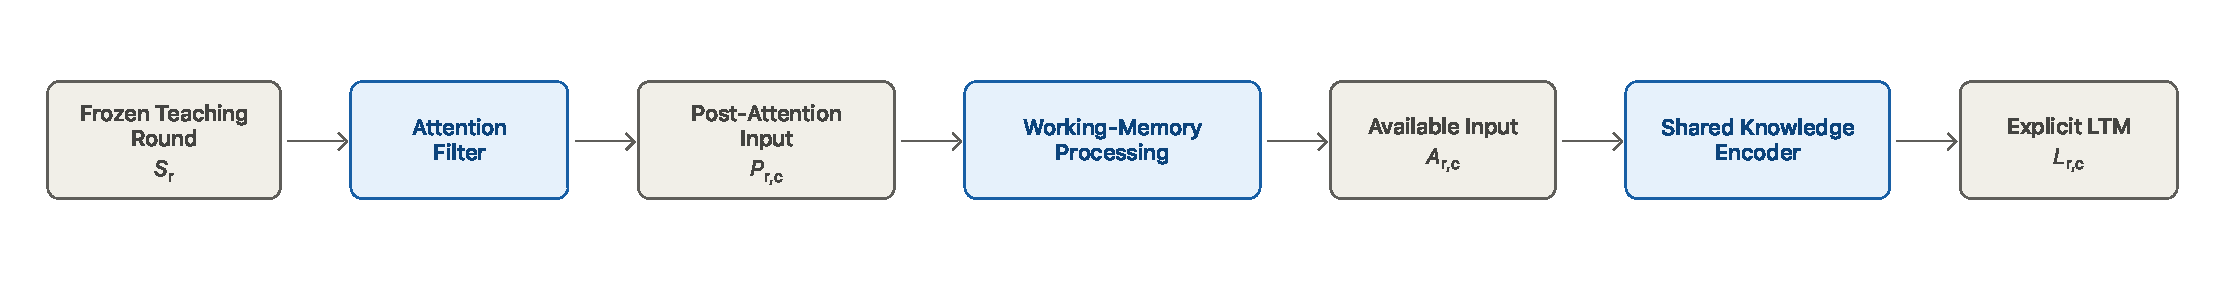
\includegraphics[width=\textwidth,keepaspectratio]{Figures/Chapter3/export/ch03_cpb_learning_information_flow.pdf}
    \caption{CPB information flow during the teaching phase.}
    \label{fig:cpb-learning-information-flow}
\end{figure}

During the assessment phase, the CPB learner no longer has access to the original instructional material. Instead, as shown in Figure~\ref{fig:cpb-assessment-phase-flow}, each response is generated solely from the accumulated Explicit Long-Term Memory and the current assessment question through LTM-Constrained Answering.

\begin{figure}[H]
    \centering
    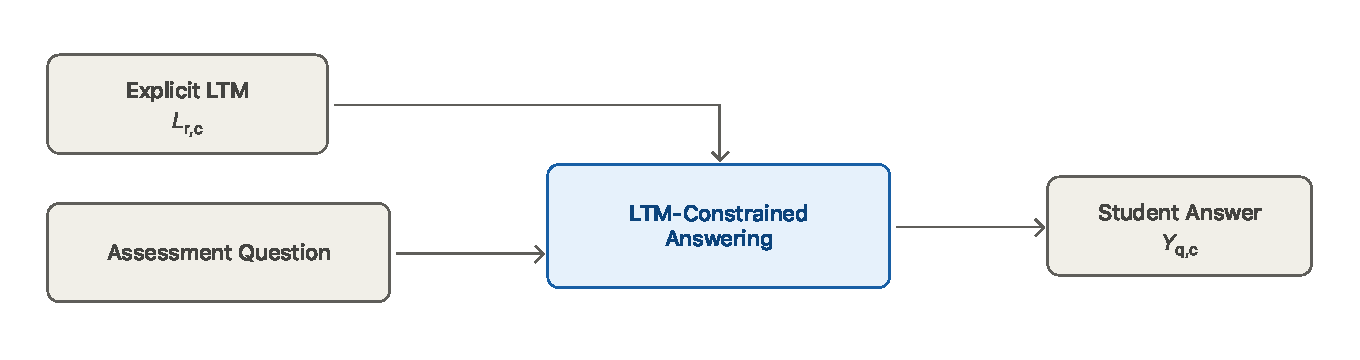
\includegraphics[width=0.88\textwidth,keepaspectratio]{Figures/Chapter3/export/ch03_cpb_assessment_phase_flow.pdf}
    \caption{CPB information flow during the assessment phase.}
    \label{fig:cpb-assessment-phase-flow}
\end{figure}

The CPB learning process can therefore be expressed as the continuous transformation \(S_r \rightarrow P_{r,c} \rightarrow A_{r,c} \rightarrow L_{r,c}\). Attention and Working Memory constitute the principal ADHD-related experimental constraints, whereas Knowledge Encoding is held constant as a shared downstream stage.

\subsection{Attention Filter}

\subsubsection{Theoretical Motivation and Functional Role}

ADHD-related attentional difficulties are frequently associated with increased susceptibility to task-irrelevant or salient stimuli. Aboitiz et al. (2014) \cite{aboitiz2014irrelevant} characterise distractibility as an important manifestation of ADHD: during a goal-directed task, attention is more likely to shift towards stimuli unrelated to the current behaviour, reflecting reduced control over irrelevant information. Experimental evidence provides corresponding support. For example, Gumenyuk et al. (2005) \cite{gumenyuk2005electrophysiological} found that introducing task-irrelevant novel sounds during a visual discrimination task produced more omission responses among children with ADHD, together with event-related potential differences associated with atypical involuntary attentional control. Similarly, Schneidt et al. (2018) \cite{schneidt2018distraction} reported greater behavioural distractibility among adults with ADHD and showed that distractor processing was moderated by task difficulty. Taken together, these findings indicate that ADHD-related attentional differences can manifest as heightened susceptibility to external distraction.

However, the available evidence does not support reducing distraction to a uniform effect that necessarily impairs performance. Van Mourik et al. (2007) \cite{van2007distraction} found that, although children with ADHD showed an enhanced orienting response to novel sounds, these stimuli reduced omission errors under some conditions, possibly because they temporarily increased arousal and improved task performance. Subsequent research has likewise shown that task-irrelevant novel sounds can reduce omission errors, reaction times, and reaction-time variability under particular experimental conditions. The present study therefore does not assume that every distractor necessarily causes information loss in learners with ADHD. Instead, it represents \textit{susceptibility to controlled distraction} as a bounded and manipulable ADHD-related attentional characteristic. The Attention Filter is consequently not intended to simulate the complete human attentional system. It is a computational abstraction of a specific process risk: when a controlled distractor successfully triggers an attentional interruption, task-relevant instructional information associated with that event may fail to remain available for subsequent processing.

Within CPB, this characteristic is operationalised through \textit{downstream information availability}, rather than through a continuous ``attention score'' or a persona-level language instruction. The purpose is to translate a global persona description, such as ``this student is easily distracted'', into an explicit and traceable process variable: whether a predefined target instructional unit remains available for subsequent processing after the Attention mechanism is triggered in a given Teaching Round. This design is consistent with evidence connecting attention to later information prioritisation and encoding. Ortega et al. (2020) \cite{ortega2020neurocognitive}, for example, reported differences in attention-related encoding and retrieval processes among adolescents with ADHD and interpreted these findings as a failure to prioritise relevant information. These studies do not imply that a human attentional failure literally deletes instructional content. Converting affected information into an unavailable state is a study-specific computational operationalisation adopted to make the mechanism controllable and traceable.

For Teaching Round \(r\), the function of the Attention stage can be expressed as

\[
S_r \rightarrow P_{r,c},
\]

where \(S_r\) denotes the frozen instructional source and \(P_{r,c}\) denotes the information state that remains available to Working-Memory Processing under condition \(c\) after Attention processing. If \(X_r\) denotes the classroom input actually presented after distractor insertion, the transformation can be represented more specifically as

\[
X_r
\xrightarrow{\mathrm{Attention}}
P^{A}_{r,c}.
\]

The scope of the Attention Filter is limited to determining which instructional information can continue into downstream processing. It does not directly create or modify Explicit Long-Term Memory, determine the final assessment answer, or dynamically select instructional content according to a later assessment question. This functional boundary represents Attention as an independent and inspectable information-state transition within the CPB pipeline. The following section describes how the mechanism is implemented through the frozen distractor-to-target mapping and a condition-specific trigger rule.

\subsubsection{Attention Filter Implementation}

The Attention Filter operates at the level of an individual Teaching Round. For each round containing a predefined distractor, the system first determines whether the Attention mechanism is triggered. This decision is not made dynamically by the LLM on the basis of instructional content or learner behaviour. Instead, it is controlled entirely by the \textit{Attention trigger probability} specified in the experimental condition. If a round has no distractor assignment, Attention cannot be triggered. If a distractor is present, the trigger probability associated with the current CPB condition determines whether the target instructional information becomes unavailable.

Study 1 uses two deterministic boundary conditions. The trigger probability is 0 under Attention OFF, so distractors never cause information removal, and 1 under Attention ON, so every eligible distractor activates the Attention Filter. Study 2 instead uses graded probabilities: CPB Zero, Low, Medium, and High correspond to trigger probabilities of 0, 0.20, 0.50, and 0.80, respectively, representing progressively greater susceptibility to distraction. For conditions with probabilities between 0 and 1, trigger decisions are generated using a frozen random seed. The same experimental configuration therefore reproduces the same Attention trajectory. The condition-specific trigger probabilities and their interpretations are summarised in Table~\ref{tab:attention-trigger-probabilities}.

\begin{table}[htbp]
\centering
\caption{Condition-specific Attention trigger probabilities.}
\label{tab:attention-trigger-probabilities}
\small
\begin{tabular}{@{}p{0.29\textwidth}cp{0.43\textwidth}@{}}
\toprule
Condition & Trigger probability & Interpretation \\
\midrule
Attention OFF / CPB Zero & 0.00 & Distractors do not trigger information loss. \\
Attention ON---Study 1 & 1.00 & Every eligible distractor triggers the mechanism. \\
CPB Low & 0.20 & Low susceptibility to distraction. \\
CPB Medium & 0.50 & Moderate susceptibility to distraction. \\
CPB High & 0.80 & High susceptibility to distraction. \\
\bottomrule
\end{tabular}
\end{table}

Whether Attention is triggered and which instructional information is affected after a trigger are implemented as two independent steps. During material construction, every distractor is paired with a fixed \texttt{target\_sentence\_id}; the learner model therefore does not infer which sentence should be affected. When Attention is not triggered, the target sentence remains available. When Attention is triggered, the corresponding target sentence is marked as unavailable and, in the final implementation, is removed from the instructional input passed to downstream processing. The selection of hard deletion and its sensitivity analysis are described in Section~\ref{sec:attention-operationalisation-sensitivity}.

\begin{figure}[H]
    \centering
    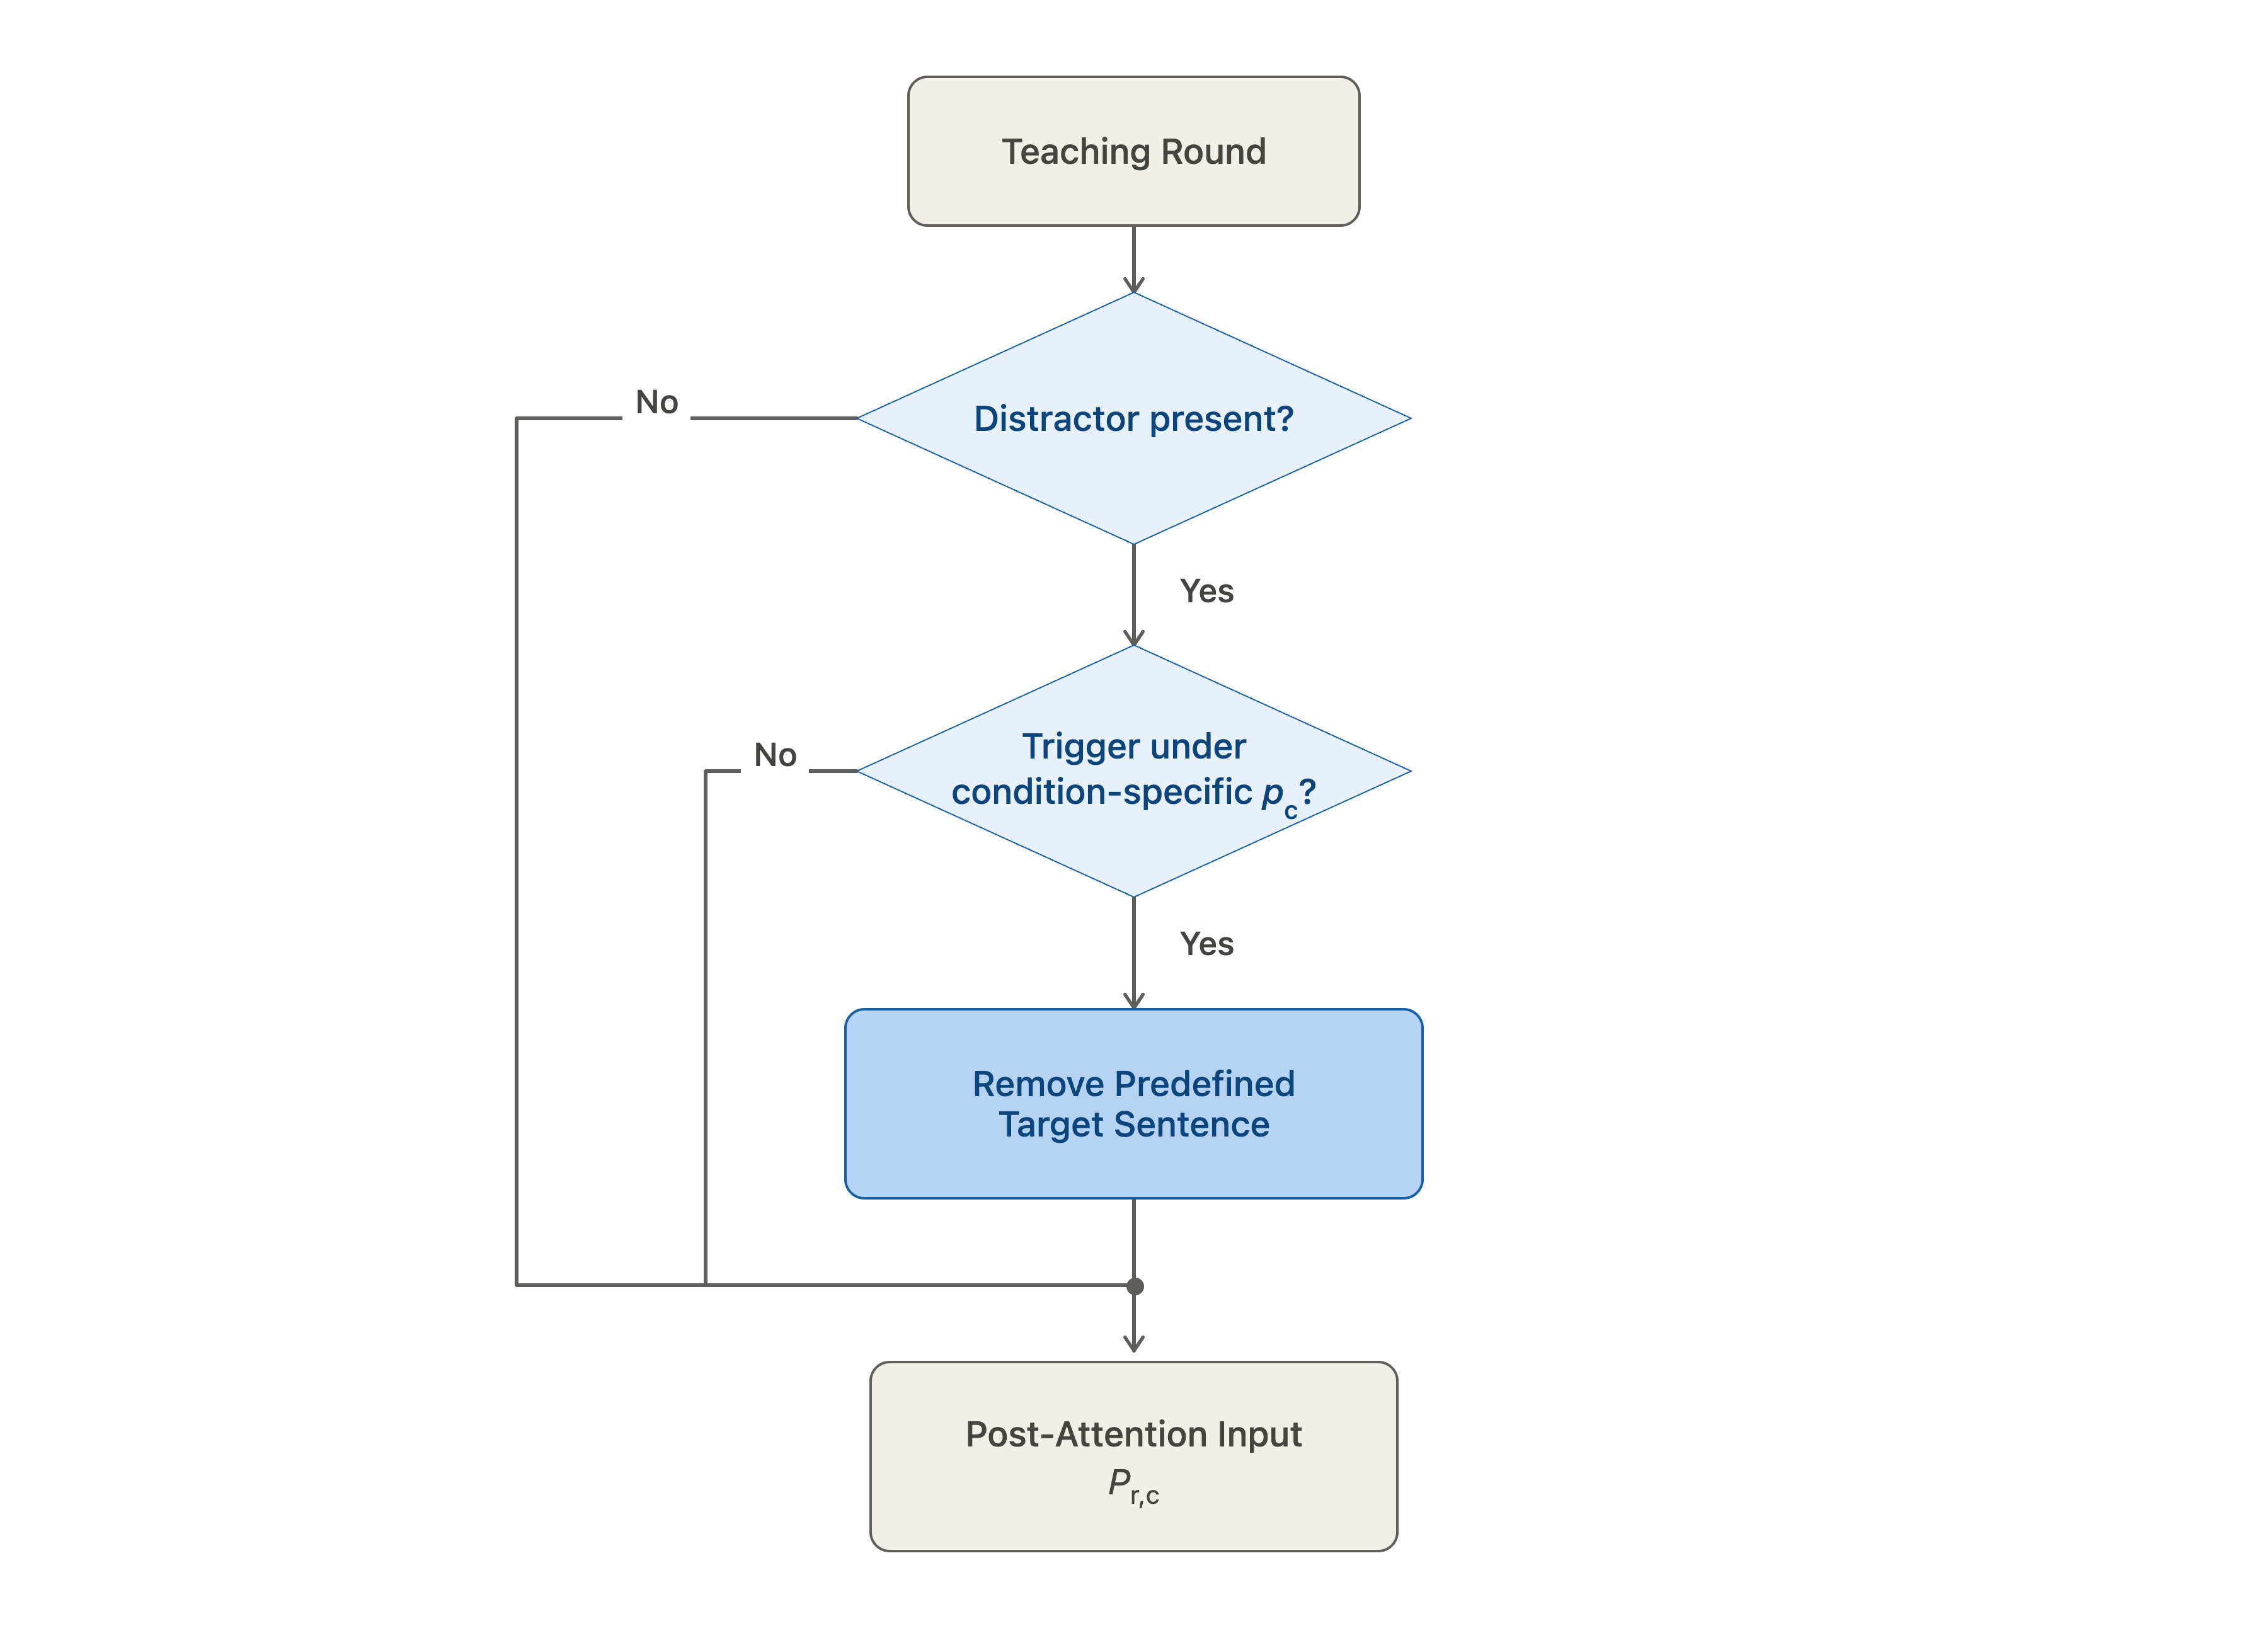
\includegraphics[width=0.62\textwidth,trim=720bp 80bp 720bp 80bp,clip,keepaspectratio]{Figures/Chapter3/export/ch03_attention_filter_decision_flow.png}
    \caption{Decision logic of the Attention Filter.}
    \label{fig:attention-filter-decision-flow}
\end{figure}

The operational logic of the Attention Filter is illustrated in Figure~\ref{fig:attention-filter-decision-flow}.

After processing, the remaining instructional information forms the post-Attention input \(P_{r,c}\), which is passed to Working-Memory Processing. The system records the trigger status, the identifier of any removed target sentence, and the resulting post-Attention input. These records support subsequent mechanism traceability and implementation-fidelity analysis.

\subsubsection{Operationalisation Sensitivity Check}
\label{sec:attention-operationalisation-sensitivity}

Direct deletion of unavailable instructional content has a clear methodological precedent in natural language processing. Feng et al. (2018) \cite{feng-etal-2018-pathologies} used input reduction to examine how input features affected model predictions by progressively removing words. Their procedure demonstrates that direct deletion is a feasible and established form of input perturbation. However, they also found that models could retain their original high-confidence predictions after the reduced inputs no longer contained sufficient semantic information for human readers. Direct deletion can therefore implement information removal unambiguously, but its downstream behavioural effect cannot be assumed to be neutral.

Lewis et al. (2020) \cite{lewis-etal-2020-bart} conducted a controlled comparison of several text-corruption strategies in BART, including token masking, token deletion, and text infilling. Token masking retained the location of missing content through a \texttt{[MASK]} token, whereas token deletion removed the corresponding token entirely. Different corruption policies produced different downstream task performance, and deletion outperformed simple masking in some generation tasks. These findings do not directly determine which unavailable-content representation should be used in CPB because BART concerns denoising pre-training rather than learner simulation. They nevertheless show that deletion and masking cannot be assumed to be behaviourally equivalent.

The present study therefore treated unavailable-content representation as an operationalisation choice requiring separate examination, rather than as an inconsequential implementation detail. The central distinction between the two candidate representation policies is summarised in Table~\ref{tab:unavailable-content-policies}. Both policies make the predefined target semantics unavailable to subsequent processing, but they represent that unavailable state differently: hard deletion removes the target sentence directly, whereas explicit masking removes its original semantics while retaining an explicit missingness cue.

\begin{table}[htbp]
\centering
\caption{Comparison of unavailable-content representation policies.}
\label{tab:unavailable-content-policies}
\small
\begin{tabular*}{\textwidth}{@{\extracolsep{\fill}}>{\raggedright\arraybackslash}p{0.16\textwidth}>{\raggedright\arraybackslash}p{0.25\textwidth}>{\raggedright\arraybackslash}p{0.23\textwidth}>{\raggedright\arraybackslash}p{0.24\textwidth}@{}}
\toprule
Policy & Representation of unavailable target & What is controlled & Additional signal \\
\midrule
Hard deletion & Target sentence removed & Target semantics unavailable & None \\
Explicit mask & Equal-character missingness marker & Same target is unavailable & Explicit cue that content is missing \\
\bottomrule
\end{tabular*}
\end{table}

Two representations of the same unavailable target information were compared. Under hard deletion, the target instructional sentence was represented as an empty value:

\[
g_{\mathrm{delete}}(s)=\emptyset.
\]

Under explicit masking, the original semantics were removed and replaced by a character-length-matched missingness marker:

\[
g_{\mathrm{mask}}(s)
=
\texttt{[CONTENT UNAVAILABLE: ...]}.
\]

The two implementations have different informational implications. Hard deletion prevents the target instructional content from entering subsequent processing, whereas explicit masking removes the original semantics while also providing an explicit meta-level cue that information is missing. Character-length matching guarantees only an identical Python character count; it does not imply an equivalent token count.

An independent sensitivity experiment tested whether this representational choice affected downstream processing using two frozen lessons (L01--L02). The experiment included three mechanism conditions in which information could become unavailable:

\begin{enumerate}
    \item Attention ON / WM OFF;
    \item Attention OFF / WM ON; and
    \item Attention ON / WM ON.
\end{enumerate}

Within this experiment, Attention ON specified a 100\% probability that the Attention Filter would be triggered. Attention OFF / WM OFF was excluded because no sentence was marked as unavailable in that condition, so the two representation policies would not produce an actual difference.

Each mechanism condition was run three times under each of the two representation policies. Each lesson contained seven frozen assessment questions: six independent questions and one cross-round integrative question. The experiment therefore produced 252 answers and 126 strictly matched paired comparisons. Across all 126 pairs, the Attention trigger, Attention-unavailable sentence identifiers, and the other CPB mechanism variables were identical in 100\% of cases. The two policies consequently followed the same mechanism trajectory and selected the same instructional information; the only intended difference was how unavailable content was represented. Any downstream difference therefore primarily tested the sensitivity of Knowledge Encoding and subsequent answering to this representational choice, rather than retesting the execution of Attention or WM.

The primary comparison was defined as

\[
\Delta \mathrm{Score}
=
\mathrm{Score}_{\mathrm{mask}}
-
\mathrm{Score}_{\mathrm{delete}}.
\]

To determine whether masking could be treated as a practically interchangeable implementation of deletion, a practical-equivalence margin of \(\pm 0.5\) points was specified in advance. A cluster bootstrap over the 14 frozen question clusters was used to compute a 95\% interval. Practical equivalence was supported only if

\[
\mathrm{CI}_{95\%}
\subseteq
[-0.5,+0.5].
\]

The sensitivity analysis showed that most matched outputs were unchanged across the two implementations, but practical equivalence was not established within the pre-specified margin. The overall mask-minus-deletion score difference was

\[
\begin{aligned}
\Delta &= -0.370, \\
\mathrm{CI}_{95\%} &= [-1.005,0.106].
\end{aligned}
\]

Although this interval crossed zero and therefore did not support a stable directional difference, it was not fully contained within the \(\pm 0.5\) practical-equivalence margin. In addition, 91.27\% of paired question scores were identical, while the small number of discrepant cases produced comparatively large downstream score shifts and were concentrated mainly in conditions involving the Attention manipulation.

Hard deletion was therefore selected not because the sensitivity experiment demonstrated that it was psychologically closer to human ADHD-related attention than masking, but because of the combined considerations of \textit{construct correspondence}, \textit{minimal intervention}, and the sensitivity evidence. The Attention Filter is intended to represent a state in which target instructional information is no longer available to downstream processing. Hard deletion implements this change directly, whereas explicit masking removes the target semantics while introducing an additional explicit missingness cue. Hard deletion was consequently frozen as the formal unavailable-content policy.

This choice does not imply that hard deletion has been validated as the psychological mechanism underlying human ADHD-related attentional disruption. Direct deletion reduces both target semantics and the length of the downstream instructional input and therefore remains a study-specific computational operationalisation. The present sensitivity evidence supports it only as the more direct and traceable implementation in this study, with fewer additional representational signals.

\subsection{Working-Memory Processing Capacity}

\mbox{}\par

\subsubsection{Theoretical Motivation and Functional Role}

Working memory (WM) is a capacity-limited cognitive system that temporarily maintains and processes task-relevant information during ongoing activity, rather than serving only as a passive short-term store \cite{baddeley2012working}. This function is particularly important for learning because learners commonly need to retain preceding material while interpreting, comparing, and integrating new instructional input. Classroom research has likewise associated working-memory ability with performance in learning activities that require information to be maintained and processed concurrently \cite{gathercole2008working}. Instructional information that has been attended to therefore cannot be assumed to proceed without restriction into subsequent knowledge formation; the processing resources available at that moment can still constrain further processing.

Working Memory has a theoretical role in ADHD learner simulation that is distinct from Attention. ADHD-related cognitive differences are not limited to susceptibility to distraction. Meta-analytic evidence also indicates reliable group-level performance differences across multiple working-memory domains between children and adolescents with ADHD and their typically developing peers \cite{martinussen2005meta,kasper2012moderators}. Further experimental research suggests that ADHD-related WM limitations may become more pronounced as cognitive load increases. Kofler et al. (2010) found that attentive behaviour was affected when storage and rehearsal demands exceeded available capacity, and that this capacity exceedance occurred at a relatively lower cognitive load among children with ADHD \cite{kofler2010adhd}. This result supports the use of a \textit{demand-sensitive capacity constraint} in CPB, rather than modelling WM-related information loss as a fixed effect independent of instructional demand.

These findings do not imply that every individual with ADHD possesses a fixed and literally smaller memory space. They instead support a stable group-level association between ADHD and limitations in working-memory performance. The present study therefore treats distraction-related information loss represented by the Attention Filter and post-Attention processing constraints as two functionally distinct mechanisms. Attention determines whether instructional information remains available after distraction, whereas WM determines whether the remaining information can continue to be processed under limited processing capacity.

On this theoretical basis, CPB represents WM as a \textit{processing-capacity constraint between Attention and Knowledge Encoding}. For Teaching Round $r$ under condition $c$, the Attention Filter first produces the post-Attention input $P_{r,c}$. The Working-Memory stage then further restricts which parts of that input can proceed to Knowledge Encoding, producing the Available Input $A_{r,c}$:

\[
P_{r,c}
\xrightarrow{\mathrm{Working\ Memory}}
A_{r,c}.
\]

Within CPB, Attention therefore determines which instructional information remains available after distraction, while WM determines whether that remaining information can proceed under the current processing constraint. The WM mechanism does not attempt to estimate a learner's physiological working-memory capacity, directly generate Explicit Long-Term Memory, or alter the final assessment answer. Its role is limited to controlling the instructional information that reaches the shared Knowledge Encoder. Section~\ref{sec:wm-mechanism-implementation} specifies how this processing-capacity constraint is implemented through instructional processing demand, condition-specific capacity thresholds, and the associated information-restriction rule.

\subsubsection{Working-Memory Mechanism Implementation}
\label{sec:wm-mechanism-implementation}

\begin{figure}[H]
    \centering
    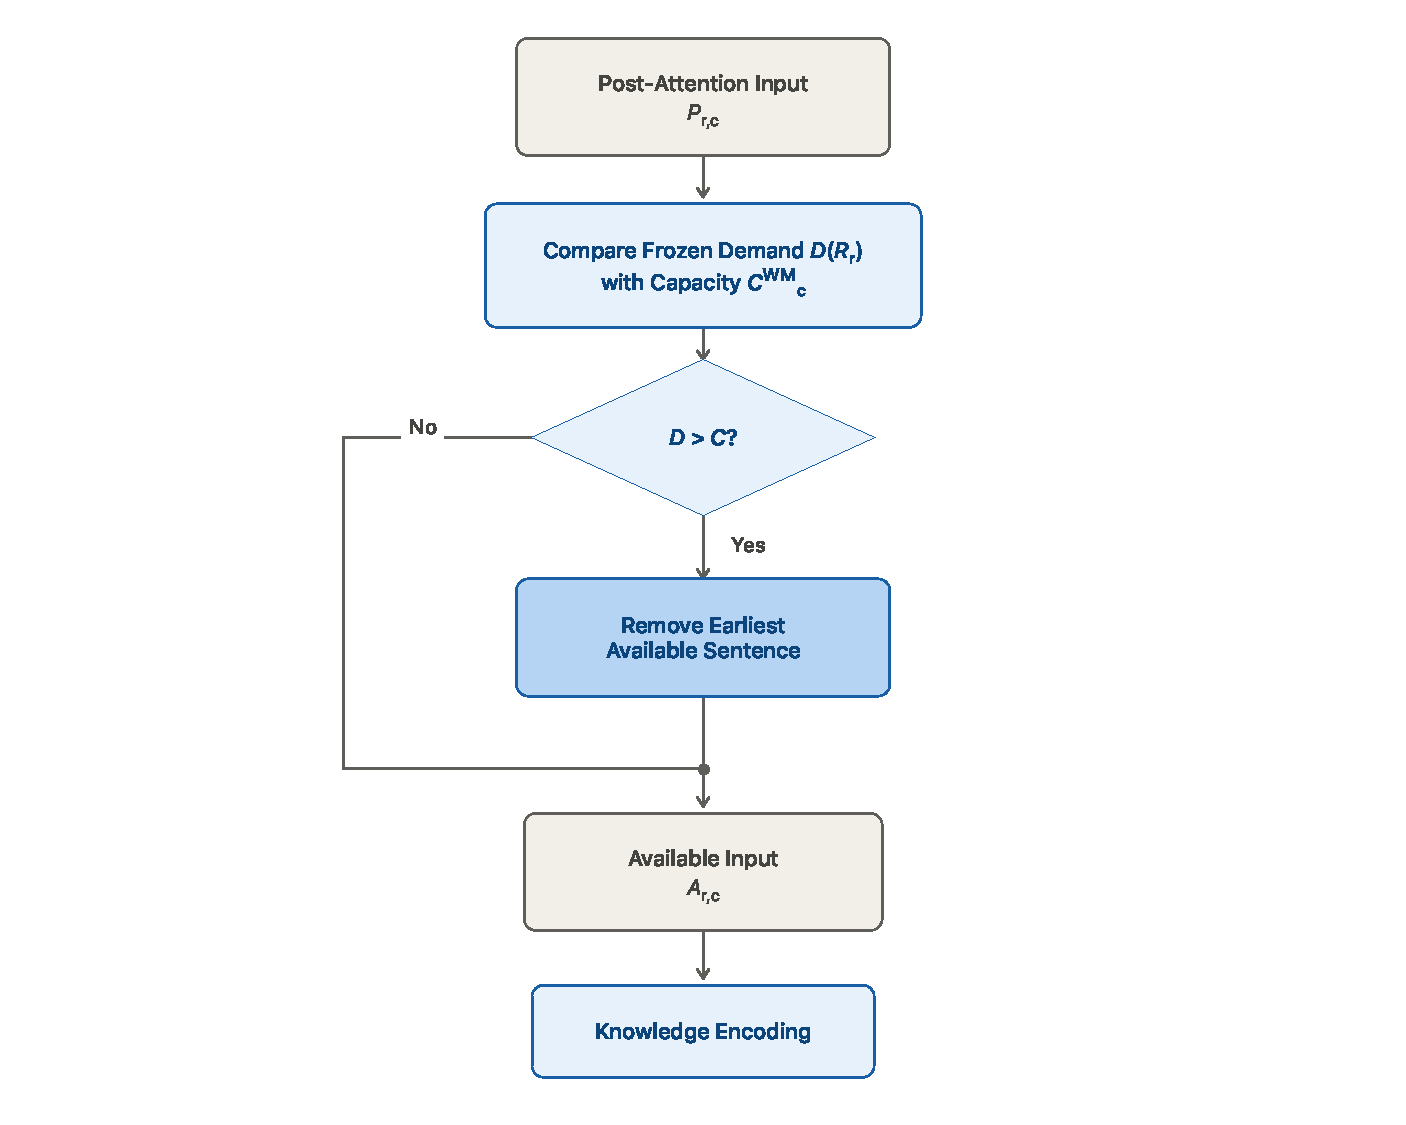
\includegraphics[width=0.72\textwidth,keepaspectratio]{Figures/Chapter3/export/ch03_working_memory_mechanism_flow.pdf}
    \caption{Decision logic of the Working-Memory mechanism.}
    \label{fig:working-memory-mechanism-flow}
\end{figure}

As illustrated in Figure~\ref{fig:working-memory-mechanism-flow}, the Working-Memory stage operates after the Attention Filter and processes one Teaching Round at a time. For Teaching Round $R_r$, the mechanism receives two inputs: the instructional information that remains available after Attention, $P_{r,c}$, and the precomputed and frozen Processing Demand Bits $D(R_r)$ for that round. PDB is a condition-invariant property of a Teaching Round: it remains identical across learner conditions and is not recalculated after Attention has made part of the input unavailable.

Within each Teaching Round, the WM trigger applies a uniform and deterministic threshold rule:

\[
\operatorname{WMOverflow}(R_r,c)
=
\mathbf{1}
\left[
D(R_r)>C^{WM}_c
\right].
\]

The WM constraint is therefore triggered when the frozen round-level processing demand is strictly greater than the WM capacity registered for the current condition; it is not triggered when demand is equal to or below capacity. Unlike the probability-based Attention trigger, WM does not involve random sampling. Consequently, the trigger decision remains identical whenever the Teaching Round, PDB value, and capacity threshold are unchanged.

When WM overflow is triggered, the mechanism restricts only the instructional sentences that remain available after the Attention stage. Let $P_{r,c}$ denote the post-Attention input. If at least one instructional sentence remains available, the system selects the earliest such sentence in the original instructional order, marks it as WM-unavailable, and applies the same hard-deletion policy used by the Attention Filter:

\[
R^{WM}_{r,c}
=
\{\operatorname{First}(P_{r,c})\}.
\]

The Available Input passed to the Knowledge Encoder is then defined as

\[
A_{r,c}
=
P_{r,c}
-
R^{WM}_{r,c}.
\]

At most one sentence-level removal is performed in each Teaching Round, and the mechanism does not remove a sentence that has already been marked as unavailable by Attention. The rule is therefore more accurately described as a \textit{deterministic, within-round FIFO-style information-restriction rule} than as a direct simulation of human Working Memory.

Each experimental condition $c$ has a prespecified WM capacity threshold $C^{WM}_c$. The threshold uses the same numerical scale as PDB, but does not represent a literal number of sentences, tokens, or working-memory slots that a real learner can retain. Instead, it is a study-specific parameter controlling the strength of the WM constraint. Lower capacity thresholds cause more Teaching Rounds to exceed the capacity boundary and therefore represent stronger WM constraints. The frozen parameters used across the experimental conditions are summarised in Table~\ref{tab:wm-capacity-thresholds}.

\begin{table}[H]
\centering
\caption{Registered Working-Memory capacity thresholds.}
\label{tab:wm-capacity-thresholds}
\footnotesize
\begin{tabular*}{\textwidth}{@{\extracolsep{\fill}}>{\raggedright\arraybackslash}p{0.17\textwidth}>{\centering\arraybackslash}p{0.14\textwidth}>{\centering\arraybackslash}p{0.22\textwidth}>{\raggedright\arraybackslash}p{0.34\textwidth}@{}}
\toprule
Condition & WM capacity $C^{WM}_c$ (bits) & Calibration on 42 source rounds & Interpretation \\
\midrule
WM OFF / CPB Zero & $10^{10}$ & 0/42 above capacity & Effectively non-binding capacity; WM removal is disabled. \\
WM ON & 321.9937895 & 21/42 above capacity & Median boundary used for binary WM mechanism validation. \\
CPB Low & 362.0988065 & 14/42 above capacity & Relatively weak WM constraint; the highest-demand one-third exceed capacity. \\
CPB Medium & 321.9937895 & 21/42 above capacity & Intermediate WM constraint; approximately one-half exceed capacity. \\
CPB High & 246.9297100 & 28/42 above capacity & Strong WM constraint; the highest-demand two-thirds exceed capacity. \\
\bottomrule
\end{tabular*}
\end{table}

The labels CPB Low, CPB Medium, and CPB High denote \textit{constraint severity}, rather than the numerical magnitude of capacity. Registered capacity therefore decreases as the WM constraint becomes stronger:

\[
C^{WM}_{\mathrm{Low}}
>
C^{WM}_{\mathrm{Medium}}
>
C^{WM}_{\mathrm{High}}.
\]

\begin{figure}[H]
    \centering
    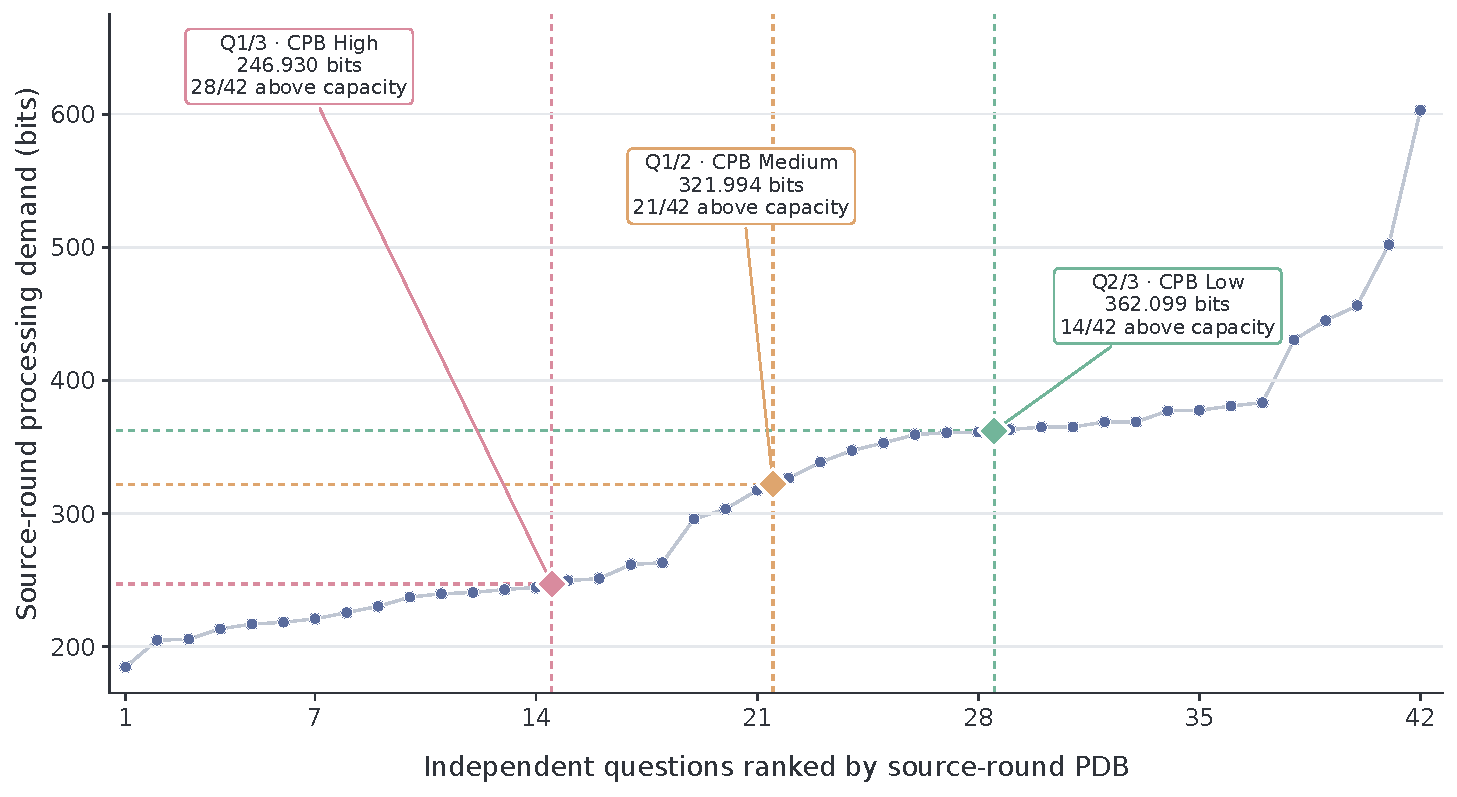
\includegraphics[width=0.86\textwidth,keepaspectratio]{Figures/Chapter3/export/Design_Figure_WM_capacity_threshold_calibration.pdf}
    \caption{Calibration of the graded Working-Memory capacity thresholds.}
    \label{fig:wm-capacity-threshold-calibration}
\end{figure}

As shown in Figure~\ref{fig:wm-capacity-threshold-calibration}, the Low, Medium, and High thresholds were selected from the frozen PDB distribution of the source rounds associated with the 42 independent assessment questions. They were fixed as WM capacity boundaries such that 14/42, 21/42, and 28/42 source rounds, respectively, exceeded the corresponding threshold. This calibration creates a progressively stronger WM-constraint gradient over the same set of assessment-relevant source rounds, allowing subsequent experiments to compare the effects of processing-capacity constraints while holding the instructional materials constant.

\subsection{Knowledge Encoding}

\subsubsection{Theoretical Motivation and Functional Role}

The primary reason for introducing a Knowledge Encoding stage is that information that remains available after Attention and Working-Memory processing should not be treated as equivalent to durable knowledge that has already been formed. The classic levels-of-processing framework argues that subsequent retention depends not only on whether information was accessible, but also on the nature of the processing applied during encoding \cite{craik1972levels}. Experimental evidence further indicates that different encoding operations produce different levels of subsequent retention, with more semantic and elaborative processing generally associated with more stable later memory performance \cite{craik1975depth}. The present study therefore distinguishes between \textit{information available for encoding} and \textit{knowledge encoded into memory}: instructional information may pass through the preceding Attention and WM constraints without necessarily entering the subsequent knowledge state in a complete, equivalent, or verbatim form.

At the same time, Knowledge Encoding is not implemented as a third ADHD-specific manipulated mechanism. The existing ADHD memory literature does not establish a single encoding deficit that can be clearly separated from Attention and Working Memory and applied uniformly across tasks. Although some studies report ADHD-related encoding differences, these effects are often intertwined with attentional allocation, working-memory demand, executive control, or encoding strategy. In one experimental paradigm, for example, children with and without ADHD showed comparable accuracy under an encoding-only condition, whereas group differences became evident after working-memory demands were introduced \cite{kofler2020working}. Other work has related aspects of encoding performance to the prioritisation of relevant information and attentional allocation \cite{ortega2020neurocognitive}, while verbal-memory performance may also depend on working memory, executive control, and the use of mnemonic strategies \cite{Lundervold2019VerbalMF,laine2025role}. The present study therefore does not assume that real ADHD and NT learners possess identical encoding abilities. Instead, \textit{shared Encoding} is adopted as a controlled modelling assumption: Attention and Working Memory are the primary manipulated mechanisms, while the downstream Encoder is held constant across simulated learners. This prevents differences already represented by the upstream mechanisms from being reintroduced through a condition-specific Encoder and thereby preserves clearer mechanism attribution.

Separating current input from an explicit memory state that can be accessed later also has precedent in computational architectures. Generative Agents write an agent's experiences to a separate natural-language memory stream and use retrieval and reflection to make those memories available to subsequent behaviour \cite{park2023generative}. CoALA similarly treats modular memory components as part of a language-agent architecture and distinguishes current observations, internal memory states, and operations performed on memory \cite{sumers2023cognitive}. Retrieval-Augmented Generation (RAG) likewise distinguishes the language model's internal parametric memory from externally accessible non-parametric memory \cite{lewis2020retrieval}. These approaches neither imply that LLM-agent memory is equivalent to human long-term memory nor directly validate human knowledge-encoding processes. They nevertheless provide an architectural basis for explicitly separating current experience and current input from a subsequently accessible knowledge state, rather than retaining all information in a continuously expanding prompt context.

On this cognitive and architectural basis, CPB defines Knowledge Encoding as a shared downstream transformation following Attention and Working Memory. For Teaching Round $r$ under condition $c$, the Available Input $A_{r,c}$ denotes the instructional information that reaches the Encoder after the preceding cognitive constraints, while $L_{r,c}$ denotes the explicit knowledge state produced from that information by the shared Knowledge Encoder:

\[
A_{r,c}
\xrightarrow{\mathrm{Encoding}}
L_{r,c}.
\]

This design allows CPB to distinguish \textit{what information reaches encoding} from \textit{what knowledge is subsequently represented in memory}. Because $A_{r,c}$ and $L_{r,c}$ are not assumed to be fully equivalent, the absence of Attention- or WM-related information loss cannot be interpreted as perfect retention. The Attention OFF / WM OFF condition is therefore defined as an \textit{encoding-only reference}, rather than as a perfect-memory condition. The $L_{r,c}$ states generated across Teaching Rounds are subsequently accumulated into an externally inspectable Explicit Knowledge State, which serves as the knowledge source for memory-constrained answering during the Assessment Phase.

\subsubsection{Shared Knowledge-Encoding Mechanism}

Within CPB, Knowledge Encoding is applied independently to each Teaching Round after Attention and Working-Memory processing. For Teaching Round $r$ under condition $c$, the Encoder receives only the Available Input $A_{r,c}$ produced by the preceding mechanisms, rather than the original instructional source or complete Teaching Round. Information already marked as unavailable by Attention or WM is not reintroduced. The transformation is defined as:

\[
L_{r,c}
=
\operatorname{Encode}(A_{r,c}),
\]

where $L_{r,c}$ denotes the round-level Explicit LTM entry formed after Encoding. The upstream mechanisms therefore determine \textit{what information reaches Encoding}, while the Knowledge Encoder transforms only the information that actually reaches that stage.

To keep this transformation consistent across simulated learners and experimental conditions, the study uses a fixed, shared Knowledge-Encoding procedure. All conditions use the same Encoder model, encoding prompt, input structure, and generation configuration; Attention status, WM-constraint level, and other learner-condition metadata do not modify the Encoding instruction. Figure~\ref{fig:knowledge-encoding-prompt} presents the frozen prompt used in the formal experiments. It instructs the model to produce one brief long-term memory entry from the classroom information actually received, to preserve the principal concepts and relationships in its own words, and not to use outside knowledge or reconstruct information absent from the input. Output is restricted to a single plain-text paragraph to reduce formatting variation in the subsequent Explicit LTM representation.

\begin{figure}[H]
    \centering
    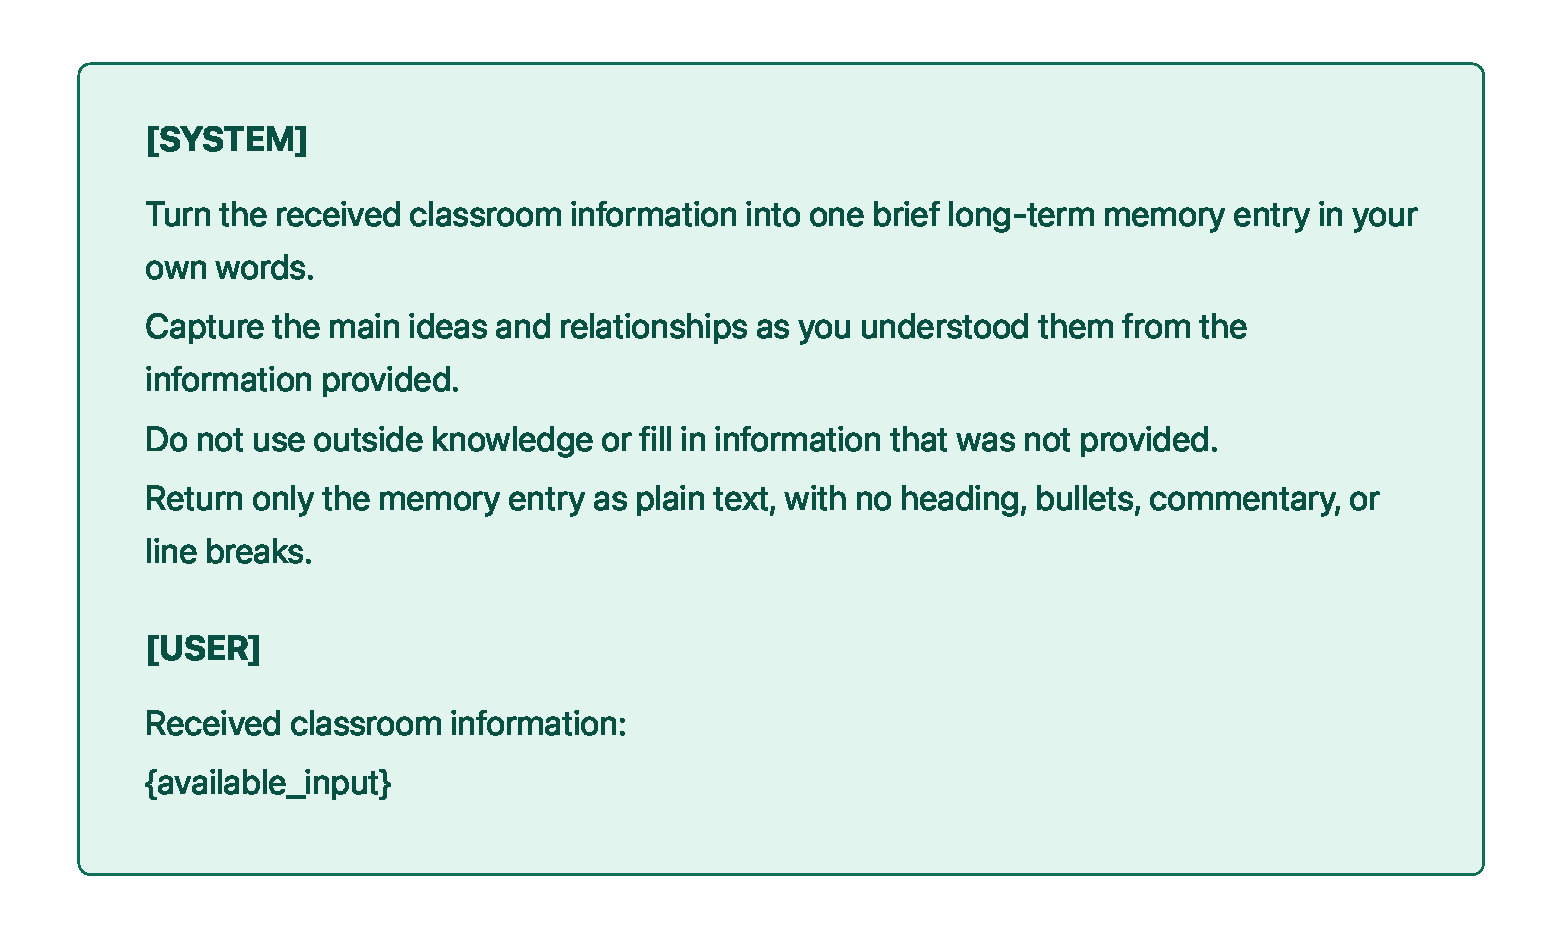
\includegraphics[width=0.88\textwidth,keepaspectratio]{Figures/Chapter3/export/ch03_knowledge_encoding_prompt_example.pdf}
    \caption{Frozen prompt used by the shared Knowledge Encoder.}
    \label{fig:knowledge-encoding-prompt}
\end{figure}

Knowledge Encoding is not intended to copy the Available Input verbatim, but to transform it into a concise semantic knowledge representation. Accordingly, $A_{r,c}$ and $L_{r,c}$ are not assumed to be identical. The Encoder may paraphrase, compress, and reorganise the input, but the resulting memory entry remains constrained by the information available in $A_{r,c}$ and should not recover instructional content that became unavailable upstream. Figure~\ref{fig:knowledge-encoding-example} illustrates this transformation: the Available Instructional Input $A_{r,c}$ appears on the left, and the encoded knowledge produced from that input appears on the right. The example shows that the central concepts and relationships can be retained while wording and compression differ from the source representation.

\begin{figure}[H]
    \centering
    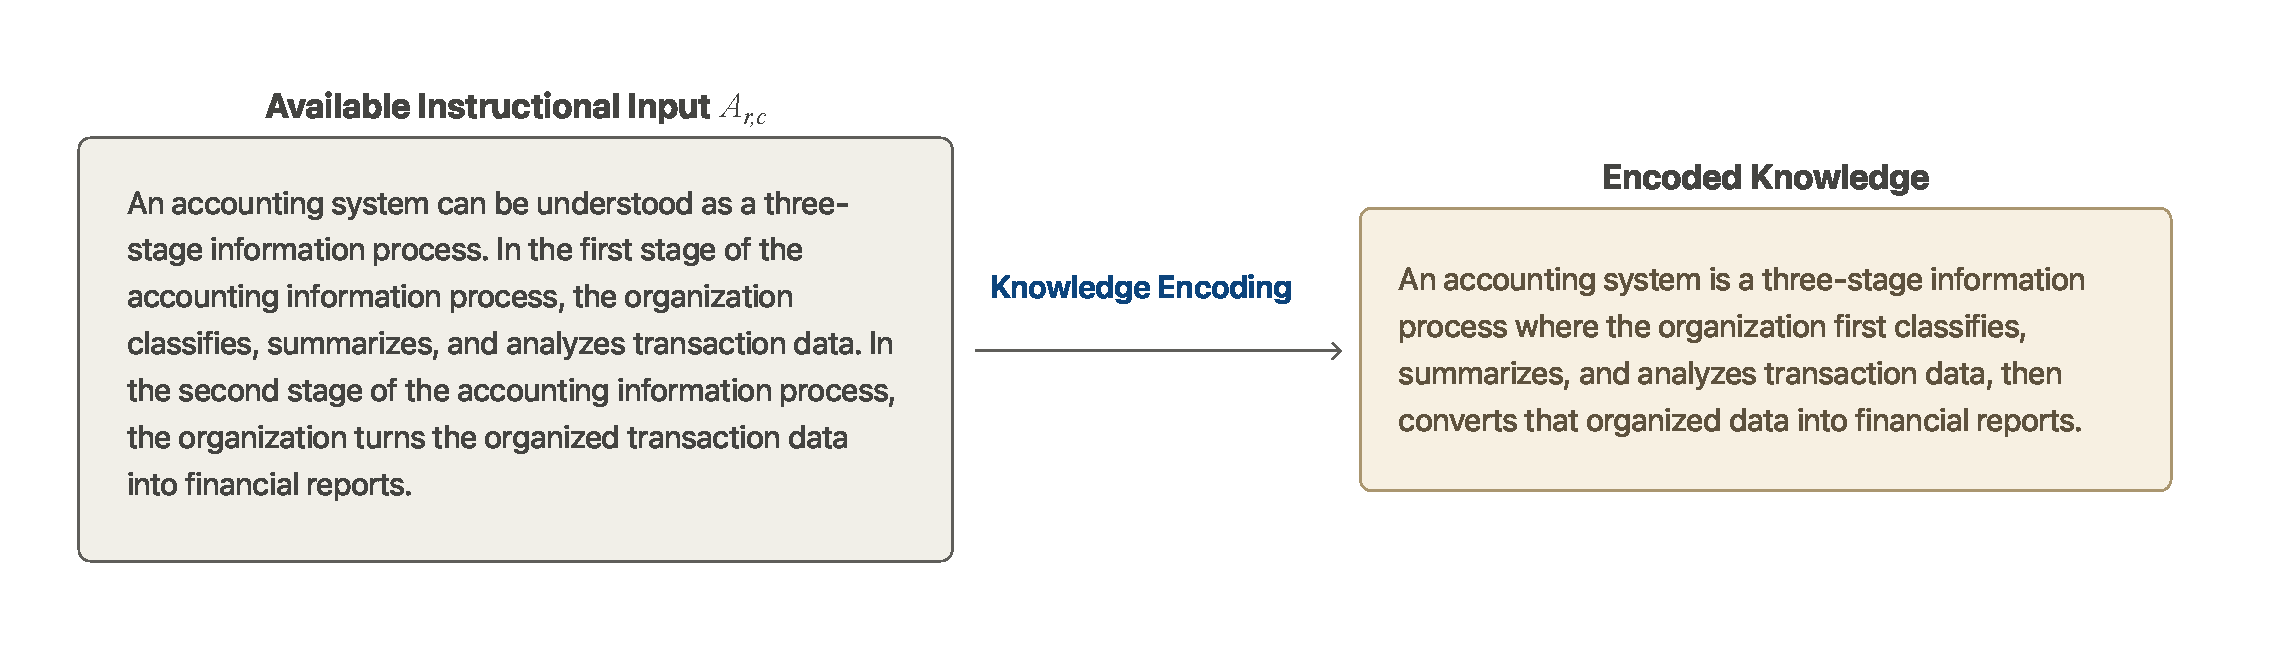
\includegraphics[width=0.96\textwidth,keepaspectratio]{Figures/Chapter3/export/ch03_knowledge_encoding_example.pdf}
    \caption{Example transformation from Available Instructional Input to encoded knowledge.}
    \label{fig:knowledge-encoding-example}
\end{figure}

The procedure is executed independently for every Teaching Round and produces at most one corresponding $L_{r,c}$. If no instructional information remains available after Attention and WM processing, such that $A_{r,c}=\emptyset$, the round does not generate a new instructional memory from distractor content, prompt context, or the model's pretrained knowledge. This rule ensures that Explicit LTM originates only from information that remains available after the preceding cognitive-processing stages and preserves a traceable relationship between Available Input and encoded knowledge.

Keeping the Knowledge Encoder shared across all experimental conditions is a controlled modelling decision, rather than an empirical claim that real ADHD and NT learners have identical encoding ability. Fixing the $A_{r,c}\rightarrow L_{r,c}$ procedure means that the principal condition differences arise from the Attention and Working-Memory mechanisms that determine which information reaches Encoding, without introducing additional condition-specific Encoder behaviour. Because Encoding remains a semantic transformation, the Attention OFF / WM OFF condition is still interpreted as an \textit{encoding-only reference}, rather than as a perfect-memory condition. The $L_{r,c}$ entries generated across Teaching Rounds are accumulated and frozen as the simulated learner's Explicit Knowledge State for memory-constrained answering during assessment.

\subsubsection{Pretrained-Knowledge and Memory-Constrained Answering}

In the formal experiments, the CPB Assessment Phase requires the simulated learner to answer questions using only the Explicit LTM formed during teaching. However, an LLM already contains pretrained knowledge, creating two alternative explanations that must first be examined. First, the student model might answer most assessment questions without exposure to any course material, thereby reducing the observable space for subsequent learning manipulations. Second, even when Explicit LTM is provided and the prompt requires memory-only answering, the model might bypass this restriction and use pretrained financial knowledge to complete its answers. The study therefore conducted a \textit{Question-Only Baseline} and a \textit{Biology-Memory-Only Control}.

In the Question-Only Baseline, DeepSeek V4-Flash received no course material, teaching history, or Explicit LTM and answered the 49 financial questions in the formal assessment set directly. The resulting answers were scored by the same Qwen3.7-Max Judge used in the formal experiments. The mean score was:

\[
\bar{S}_{\mathrm{Baseline}}=7.823.
\]

This result indicates that DeepSeek V4-Flash already possesses financial-domain pretrained knowledge, so formal assessment performance cannot be assumed to originate entirely from the Teaching Phase. At the same time, the baseline remained below the maximum score of 10, leaving observable learning headroom in the assessment set.

Figure~\ref{fig:memory-restriction-prompt} presents the frozen Memory Restriction and Core Student Instruction used during assessment. The prompt requires every factual claim to be supported by the provided learned memory, permits only meaning-preserving paraphrase, and directs the learner to report when information was not retained rather than complete missing knowledge from other sources.

\begin{figure}[H]
    \centering
    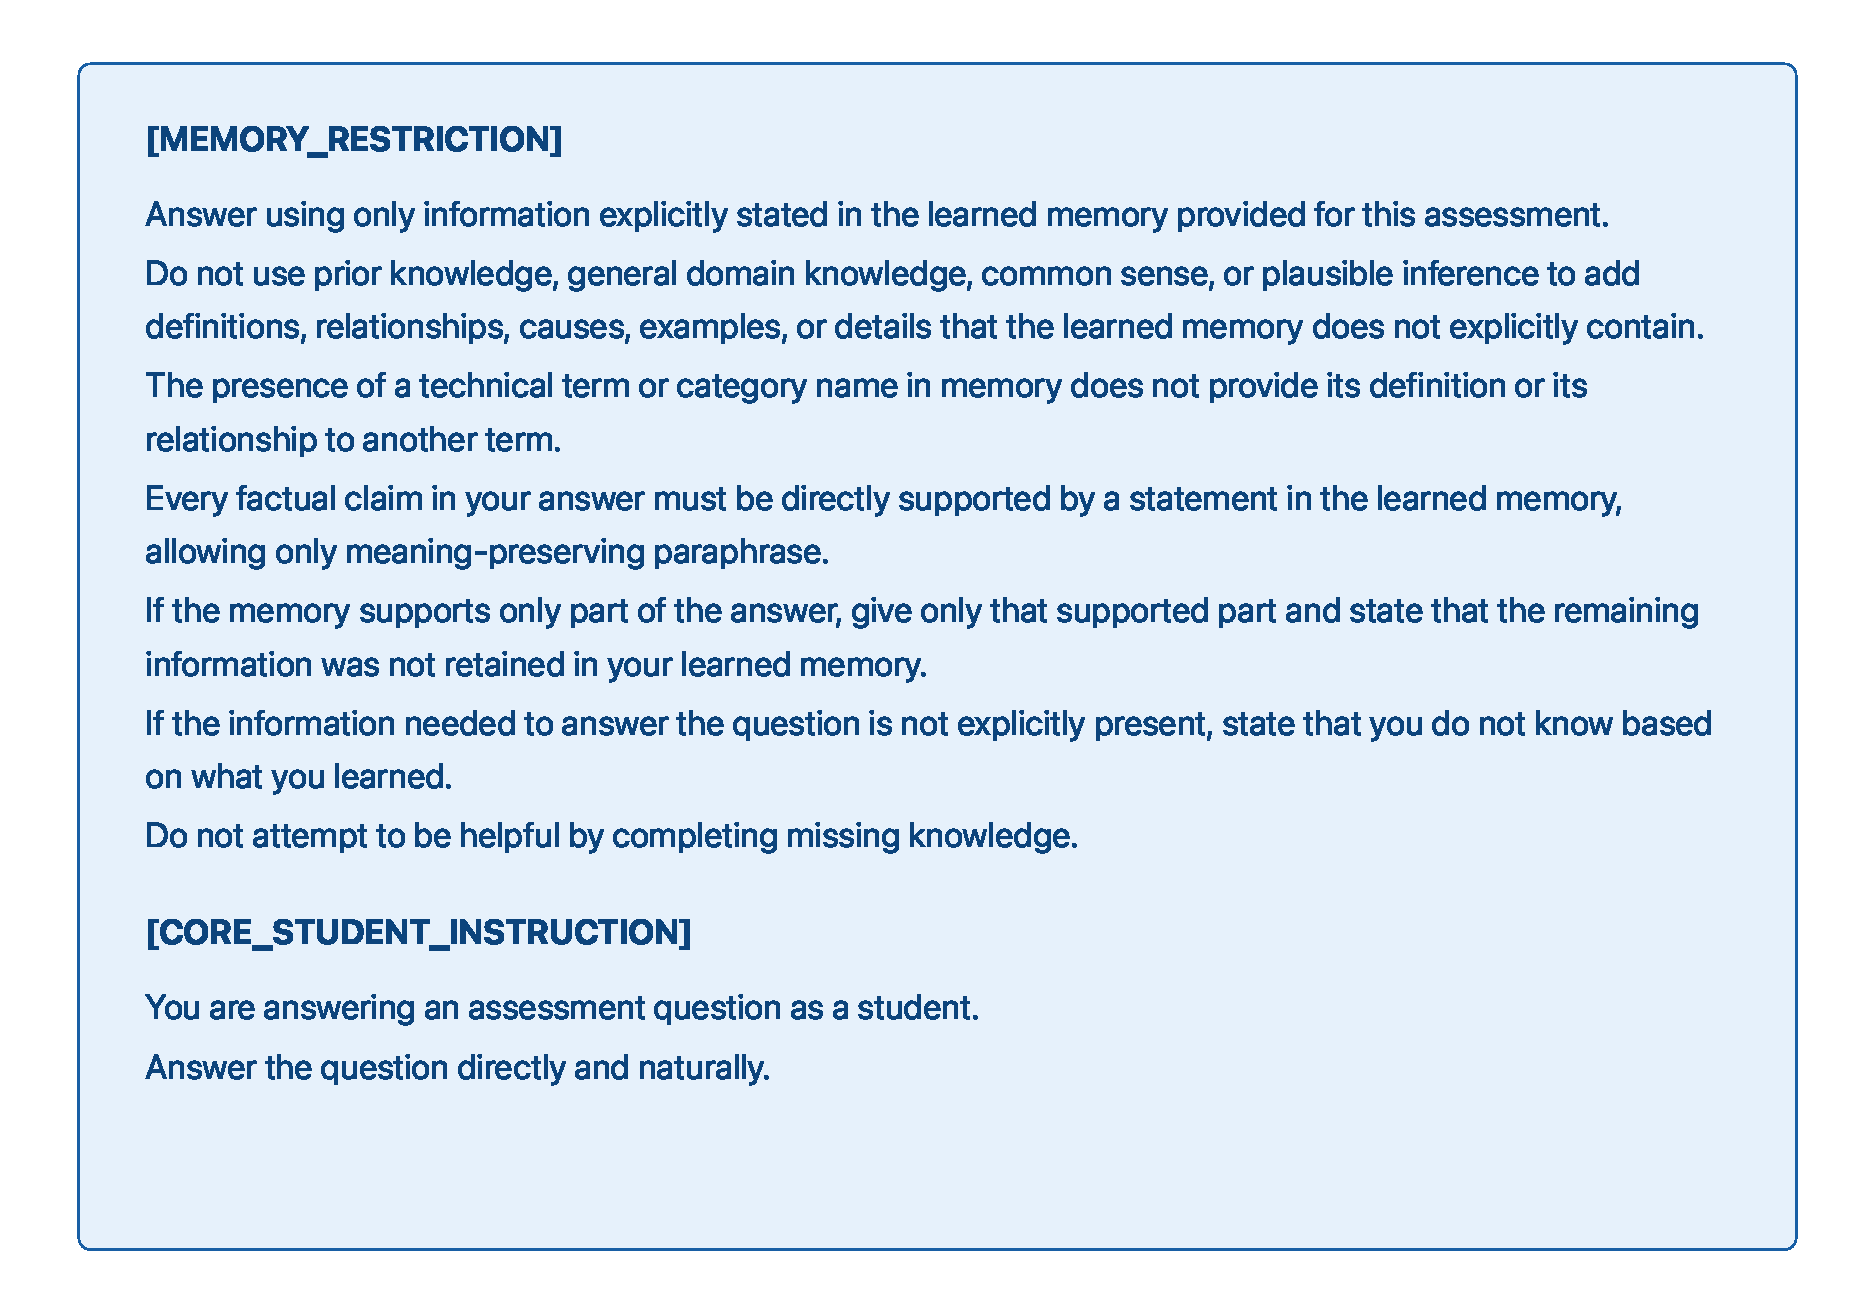
\includegraphics[width=0.92\textwidth,keepaspectratio]{Figures/Chapter3/export/ch03_memory_restriction_prompt_example.pdf}
    \caption{Memory-restriction and core student instructions used during assessment.}
    \label{fig:memory-restriction-prompt}
\end{figure}

To test whether this restriction could operationally constrain the model's information source, the study constructed a Biology Explicit LTM unrelated to the financial course and substituted it for the Explicit LTM formed from the course materials. The biology memory contained 14 entries and 702 words covering cells, genetics, physiology, evolution, and ecology, without financial, accounting, market, or investment content. DeepSeek V4-Flash then answered the same 49 financial assessment questions under the formal memory-constrained answering prompt. All answers were scored by the same Qwen3.7-Max Judge against the frozen set of 137 atomic criteria.

Table~\ref{tab:pretrained-memory-controls} summarises the control results. The Biology-Memory-Only condition produced a mean score of zero, compared with 7.823 in the unrestricted Question-Only Baseline.

\begin{table}[H]
\centering
\caption{Pretrained-knowledge baseline and memory-restriction control results.}
\label{tab:pretrained-memory-controls}
\begin{tabular}{lr}
\hline
\textbf{Condition} & \textbf{Mean Score} \\
\hline
Question-Only Baseline & 7.823 \\
Biology Memory Only & 0.000 \\
Difference & $-7.823$ \\
\hline
\end{tabular}
\end{table}

Under Biology Memory Only, all 49 assessment questions received a final score of zero. The Judge classified all 137 rubric criteria as \texttt{Absent}, with \texttt{Correct = 0} and \texttt{Contradicted = 0}; mean scores were also zero for the questions associated with each of the seven lessons. This creates a clear contrast: without memory restriction, the model used pretrained knowledge to obtain a relatively high score on financial questions, whereas supplying an Explicit LTM with no relevant financial information and requiring memory-only answering reduced the score to zero.

The result supports the \textit{operational validity of the memory-access restriction in the current student-model setting}. More precisely, when the supplied Explicit LTM lacked the information required by an assessment question, DeepSeek V4-Flash did not exhibit correct completion from pretrained financial knowledge under the current answering prompt. The control therefore verifies that compliance with the instruction to answer only from the supplied memory behaved as intended; it does not imply that the model's internal pretrained knowledge was removed or rendered inaccessible.

On the basis of these controls, the formal assessment procedure treats the frozen Explicit Knowledge State as the simulated learner's only experimental knowledge source. For condition $c$, the round-level LTM entries formed across Teaching Rounds are accumulated and frozen as:

\[
\mathcal{L}_c=
\{L_{1,c},L_{2,c},\ldots,L_{R,c}\}.
\]

Each assessment question $Q_q$ is answered independently from the same frozen Explicit Knowledge State:

\[
\mathcal{L}_c + Q_q
\rightarrow
Y_{q,c}.
\]

The original instructional source, complete teaching history, and information previously made unavailable by Attention or Working Memory are not supplied to the answering model. Knowledge Encoding and question answering represent, respectively, the knowledge-formation and knowledge-use stages of the same simulated learner. Because the corresponding Encoding and Memory Restriction prompts behaved stably with DeepSeek V4-Flash, the formal experiments use DeepSeek V4-Flash at both stages to avoid introducing additional cross-model differences.

Taken together, the Question-Only Baseline shows that the assessment set was not fully mastered by the student model without teaching exposure and therefore retained observable learning headroom. The Biology-Memory-Only Control shows that answer generation could be effectively constrained by the provided Explicit LTM under the current prompt and model configuration. These controls strengthen the attribution of subsequent performance differences to the learning-process manipulations and the Explicit Knowledge States they produced, rather than to unrestricted use of pretrained financial knowledge during assessment.

\section{Research Design and Evaluation Strategy}

\subsection{Research Questions and Study Mapping}

The overall research question guiding this study is:

\begin{quote}
\textbf{Main RQ:} Can a cognitive-process-based representation provide a more theory-consistent, traceable, and robust basis for simulating ADHD-related learning behaviour than persona prompting alone?
\end{quote}

This overarching question is addressed through three research questions with distinct evidential roles:

\begin{quote}
\textbf{RQ1---Mechanism:} Does the CPB processing pipeline produce intended and traceable transitions from instructional information, through attention, working-memory processing and encoding, to the downstream knowledge state?

\textbf{RQ2---Representation:} Compared with persona prompting, does CPB produce learning behaviour that shows more theoretically consistent sensitivity to controlled distraction and processing demand?

\textbf{RQ3---Multidimensional Robustness:} When additional functionally heterogeneous learner characteristics are introduced, does a factorised CPB representation maintain learning outcomes more consistently than joint persona prompting?
\end{quote}

The three research questions are examined through a progressive experimental design. Study 1 first evaluates whether the internal CPB mechanisms operate as intended and produce traceable information-state transitions. Study 2 then compares CPB with persona prompting under controlled distraction and instructional processing demand. Finally, Study 3 introduces additional heterogeneous learner characteristics to examine the robustness of joint and factorised representations. Table~\ref{tab:rq-study-mapping} summarises the mapping between research questions, evidential roles, experimental studies, and the primary forms of evidence used to address each question.

\begin{table}[H]
\centering
\caption{Mapping of research questions to experimental studies and evidence.}
\label{tab:rq-study-mapping}
\small
\setlength{\tabcolsep}{3pt}
\renewcommand{\arraystretch}{1.2}
\begin{tabular}{p{0.06\textwidth} p{0.20\textwidth} p{0.39\textwidth} p{0.28\textwidth}}
\toprule
\textbf{RQ} & \textbf{Evidential role} & \textbf{Study and core comparison} & \textbf{Primary evidence} \\
\midrule
\textbf{RQ1} & Mechanistic validity & \textbf{Study 1:} $2 \times 2$ Attention OFF/ON $\times$ WM OFF/ON ablation, with a shared Encoding stage and A0W0 as an encoding-only reference & Correct mechanism execution and traceable information-state changes \\
\textbf{RQ2} & Comparative representational validity & \textbf{Study 2:} Prompt-NT, Prompt-ADHD, CPB Zero, Low, Medium and High under matched distraction and instructional processing-demand conditions & Systematic sensitivity to distraction and processing demand \\
\textbf{RQ3} & Representational robustness & \textbf{Study 3:} Matched aligned and conflicting multidimensional learner profiles under joint persona prompting and factorised CPB representation & Preservation of cognitive-constraint structure and localisation of cross-attribute effects \\
\bottomrule
\end{tabular}
\end{table}

\subsection{Study 1---Mechanistic Validity of CPB}

\mbox{}\par

\subsubsection{Research Question and Expected Patterns}

\mbox{}\par

\subsubsection{Experimental Design and Conditions}

\mbox{}\par

\subsubsection{Evaluation Measures and Planned Analysis}

\mbox{}\par

\subsection{Study 2---Comparative Representational Validity}

\mbox{}\par

\subsubsection{Research Question and Expected Patterns}

\mbox{}\par

\subsubsection{Experimental Design and Conditions}

\mbox{}\par

\paragraph{A. Persona-Prompted Conditions}

\mbox{}\par

\paragraph{B. Graded CPB Conditions}

\mbox{}\par

\subsubsection{Evaluation Measures and Planned Analysis}

\mbox{}\par

\subsection{Study 3---Multidimensional Representational Robustness}

\mbox{}\par

\subsubsection{Research Question and Expected Patterns}

\mbox{}\par

\subsubsection{Experimental Design and Conditions}

\mbox{}\par

\paragraph{A. Joint-Prompt and Contrastive Learner Profiles}

\mbox{}\par

\subsubsection{Evaluation Measures and Planned Analysis}

\mbox{}\par

\section{Implementation, Reproducibility and Ethical Scope}

\mbox{}\par

\subsection{Models and Generation Settings}

\mbox{}\par

\subsection{Experiment Execution and Reproducibility}

\mbox{}\par

\subsection{Statistical Uncertainty and Repetition Conventions}

\mbox{}\par

\subsection{Ethical Scope and Interpretation}

\mbox{}\par

%%%%%%%%%%%%%%%%%%%%%%%%%%%%%%%%%%%%%%%%%%%%%%%%%%%%%%%%%%%%%%%%%%%%%%%%%%%%%%%%
\chapter{Results} \label{Chap4}

\section{Results Overview}

\mbox{}\par

\section{RQ1---Cognitive-Mechanism Effects}

\mbox{}\par

\subsection{Attention-Filtering Effects}

\mbox{}\par

\subsection{Working-Memory Capacity Effects}

\mbox{}\par

\subsection{Combined Attention and WM Effects}

\mbox{}\par

\subsection{Source to Available Input to LTM}

\mbox{}\par

\subsection{RQ1 Summary}

\mbox{}\par

\section{RQ2---CPB versus Persona-Prompted ADHD Simulation}

\mbox{}\par

\subsection{Overall Learning Performance}

\mbox{}\par

\subsection{Sensitivity to Controlled Distraction}

\mbox{}\par

\subsection{Sensitivity to Processing Demand}

\mbox{}\par

\subsection{Independent versus Integrative Learning}

\mbox{}\par

\subsection{Error Traceability}

\mbox{}\par

\subsection{RQ2 Summary}

\mbox{}\par

\section{RQ3---Cross-Attribute Robustness}

\mbox{}\par

\subsection{Added Learner Attributes}

\mbox{}\par

\subsection{Preservation of ADHD-Related Learning Patterns}

\mbox{}\par

\subsection{Attribute Fidelity}

\mbox{}\par

\subsection{Prompt-Based versus Factorised Representation}

\mbox{}\par

\subsection{RQ3 Summary}

\mbox{}\par

\section{Summary of Findings}

\mbox{}\par

%%%%%%%%%%%%%%%%%%%%%%%%%%%%%%%%%%%%%%%%%%%%%%%%%%%%%%%%%%%%%%%%%%%%%%%%%%%%%%%%
\chapter{Conclusions and Future Work} \label{Chap5}

This study addressed a central learner-representation question: how should learner characteristics be represented in LLM-based student simulation when they are expected to influence information processing, knowledge formation, and downstream behaviour through the learning process? Using ADHD-related Attention and Working-Memory characteristics as a controlled case, the thesis compared persona prompting with a Cognitive-Process-Based (CPB) representation and reached a qualified affirmative answer to the Main Research Question. The experiments showed that CPB could translate predefined processing constraints into attributable information- and knowledge-state changes and produce task-sensitive behavioural patterns aligned with the expected directions of controlled distraction and instructional processing demand. In contrast, persona-level differences did not consistently translate into process-sensitive effects of the same kind. After Language Ability and Big-Five response-stage prompts were introduced, specific CPB assessment outcomes changed, but the existing graded constraint structure and associated aggregate patterns remained observable.

The principal contribution of this thesis is a \textbf{functionally grounded learner representation}. It separates selected process-relevant characteristics from persona instructions that directly prescribe how a student should appear, allowing those characteristics instead to alter learner state through constraints on the learning process and allowing the resulting state to influence downstream behaviour. Building on this representation, the thesis also developed a progressive validation framework aligned with the scope of its claims, moving from mechanism execution and information-state transitions to task-sensitive behaviour and attribute-extension analysis. The explicit knowledge state and process traceability therefore serve as methodological advantages of the process-based representation: they make the relationship between behavioural outcomes and the processes that produced them directly inspectable.

These conclusions remain subject to clear scope limitations. Attention and Working Memory are limited functional abstractions of ADHD cognition and do not represent a complete or clinically realistic ADHD learning process. PDB is a surprisal-based proxy for instructional processing demand rather than a direct measure of human cognitive load. The study is also limited to English finance materials, multi-round teaching, and short-answer assessment, and no real ADHD learner data were available to establish external behavioural validity. Future work should therefore validate distraction- and processing-demand-related patterns against data from real ADHD and NT learners, refine probabilistic attention allocation, partial retention, interference, and dynamic processing mechanisms, and extend the evaluation across subject domains, task formats, and base models.

Overall, this thesis does not claim that CPB should replace persona prompting in every setting. Its broader implication is that \textbf{learner representation should match the functional level at which a learner characteristic is expected to operate}. Persona prompting may be sufficient for characteristics that primarily affect linguistic expression or interaction style. For characteristics expected to alter knowledge acquisition and subsequent task behaviour through the learning process, representing them at the corresponding processing layer and allowing behavioural differences to emerge from the resulting learner state provides a direction for developing more modular and functionally grounded LLM-based simulated learners.

%%%%%%%%%%%%%%%%%%%%%%%%%%%%%%%%%%%%%%%%%%%%%%%%%%%%%%%%%%%%%%%%%%%%%%%%%%%%%%%%
\chapter{Conclusions} \label{Chap6}

% Clearly answer the main research question.
% Summarise the evidence for RQ1, RQ2, and RQ3.
% State the most important contribution without introducing new results.

%%%%%%%%%%%%%%%%%%%%%%%%%%%%%%%%%%%%%%%%%%%%%%%%%%%%%%%%%%%%%%%%%%%%%%%%%%%%%%%%
\chapter{Future Work} \label{Chap7}

% Discuss external validation with human learners, richer cognitive mechanisms,
% additional learner attributes, broader subject domains, and educational use.

%%%%%%%%%%%%%%%%%%%%%%%%%%%%%%%%%%%%%%%%%%%%%%%%%%%%%%%%%%%%%%%%%%%%%%%%%%%%%%%%
\renewcommand{\bibname}{References}
\bibliographystyle{ieeetr}
%\bibliography{Bibliography.bib}
\bibliography{references.bib}
%%%%%%%%%%%%%%%%%%%%%%%%%%%%%%%%%%%%%%%%%%%%%%%%%%%%%%%%%%%%%%%%%%%%%%%%%%%%%%%%
% APPENDIX
\begin{appendices}
\chapter{Supplementary Materials}\label{appendix:supplementary-materials}
% Add prompts, rubrics, data schemas, and supplementary results here.

\chapter{Source Code}\label{appendix:source-code}
The project source code and dissertation materials are available at:\\
\url{https://github.com/willowliu506-sys/Beyond-Persona-Prompting}


\end{appendices}
% INDEX?

\end{document}
